\documentclass[]{article}
\usepackage{amsmath}
\usepackage{amssymb}
\usepackage{fullpage}
\usepackage{biblatex}
\usepackage{graphicx}
\usepackage{float}
\usepackage[hidelinks]{hyperref}
\usepackage{multirow}
\usepackage{cellspace} 
\usepackage{amsthm}
\theoremstyle{definition}
\usepackage[framed,numbered,autolinebreaks]{mcode}
\usepackage{pgfplots} 
\newtheorem{exmp}{Ex}[section]
\newcommand*\diff{\mathop{}\!\mathrm{d}}
\newcommand*\Diff[1]{\mathop{}\!\mathrm{d^#1}}

\title{Numerical Methods for Engineers: A practical approach}
\author{Jonathan Haydak}
\numberwithin{equation}{section}
\begin{document}
	\maketitle
	\setlength\cellspacetoplimit{4pt}
	\setlength\cellspacebottomlimit{4pt}
	\tableofcontents
	\newcommand{\dydx}[2]{\frac{\text{d}{#1}}{\text{d} {#2}}}
	\newcommand{\der}[1]{\frac{\partial}{\partial {#1}}}
	\part{Differential Equations}
	\section{Derivative approximations}
	Like so many things in math, we start by taking a function $f(x)$ and expanding it around some $x = x_0$ with a taylor series:
	\begin{equation}
	f(x) = f(x_0) + f'(x_0) (x-x_0) + \frac{f''(x_0)}{2!} (x-x_0)^2 + \frac{f'''(x_0)}{3!} (x-x_0)^3 
	\end{equation}
	Neglecting the issue of convergence, we know that this expression is true for all $x$ in a small neighborhood of $x_0$. Next, if we stay within a small neighborhood of $x_0$, we see that the $(x-x_0)^2$ will be much larger than the remaining terms due to the fact that a small number repeatedly raised to higher powers rapidly approaches zero. Given this, we truncate the Taylor series and make the approximation:
	\begin{equation}
	f(x) \approx f(x_0) + f'(x_0) (x-x_0) + \mathcal{O}\left((x-x_0)^2 \right) \label{d1}
	\end{equation}
	It is worth taking a second to discuss what these equations means. Formally, it means that regardless of the choice of $x_0$, there exists a $c$ such that 
	\begin{align}
	\lvert f(x) - f_{approx}(x) \rvert \leq c \lvert x- x_0 \rvert^2 \nonumber \\
	\lvert f(x) - \left( f(x_0) + f'(x_0) (x-x_0) \right) \rvert \leq c \lvert x- x_0 \rvert^2
	\end{align}
	What this is saying is that the error in our approximation of $f(x)$ is proportional to $(x-x_0)^2$. Moreover, this says that we can make our approximation arbitrarily accurate by making $(x-x_0)^2$ small enough. In general, the exact functional form of $mathcal{O}(x-x_0)^2$ and we can play fast and dirty with algebraic manipulations involving this (and other error terms). Namely, we can multiply it by a constant, and smaller terms, and it still remains the same:
	\begin{align*}
	&\mathcal{O} (x-x_0) = \mathcal{O} (x_0 - x) \\
	&\mathcal{O}(x-x_0) = -\mathcal{O}(x-x_0) \\
	&\mathcal{O}(x-x_0) = 50\mathcal{O}(x-x_0) \\
	&\mathcal{O}(x-x_0) = \mathcal{O}(x-x_0) + (x-x_0)^3 - (x-x_0)^4 \\
	&\frac{\mathcal{O}(\left(x-x_0\right)^2)}{x-x_0} = \mathcal{O}(x-x_0) 
	\end{align*}
	and so on.
	
	Now, suppose we want to approximate $f'(x_0)$ using \eqref{d1}. This gives us:
	\begin{equation}
	f'(x_0) \approx \frac{f(x) - f(x_0)}{x-x_0} + \mathcal{O}(x-x_0)
	\end{equation}
	If we evaluate the above expression at $ x = x_0 + \Delta t$, we end up with a formula for approximating the derivative at any point $x_0$ whose error is proportional to $\Delta x$.
	\begin{equation}
	f'(x_0) \approx \frac{f(x_0+\Delta x) - f(x_0)}{\Delta x} + \mathcal{O}(\Delta x) \label{fd}
	\end{equation}
	\eqref{fd} is called a \textbf{forward difference quotient}. We say it is first order accurate in $\Delta x$ because its error is $\mathcal{O}(\Delta x)$. If instead we were to evaluate \eqref{d1} at $x = x_0 - \Delta t$, we would get a \textbf{backward difference quotient}:
	\begin{equation}
	f'(x_0) \approx \frac{f(x_0) - f(x_0-\Delta x)}{\Delta x} + \mathcal{O} (\Delta x) \label{bd}
	\end{equation}
	Can we do better though? Yes, but we have to include more terms in the approximation. For example, what if we were to average the forward and backward difference quotient. Would we end up with a more accurate approximation. If you naively add up the terms in \eqref{fd} and \eqref{fd} and divide by 2, you might be tempted to say that the error on this type of scheme is still first order. However, there is cancellation going on in the error terms that you will miss if you do not expand out the difference quotients using more terms. Using a second order taylor series, we can write out the following expansions:
	\begin{align}
	f(x+\Delta x) &= f(x) + f'(x) \Delta x + \frac{f''(x)}{2} \Delta x^2 + \mathcal{O}(\Delta x^3) \label{ tayf} \\
	f(x-\Delta x) &= f(x) - f'(x) \Delta x + \frac{f''(x)}{2} \Delta x^2 + \mathcal{O}(\Delta x^3) \label{ tayb} 
	\end{align}
	Taking \eqref{ tayf} - \eqref{ tayb} and rearranging gives the following:
	\begin{equation}
	f'(x) = \frac{f(x+\Delta x) - f(x-\Delta x)}{2\Delta x} + \mathcal{O}(\Delta x^2) \label{cd}
	\end{equation}
	\eqref{cd} is called a \textbf{central difference quotient}. It is the average of the forward and backward quotients and we see that it is second order accurate.
	
	In a similar manner to how we obtained the central difference quotient, you can obtain higher order accuracy forward, backward, and central difference quotients by writing out taylor expansions of $f(x+\Delta x)$, $f(x-\Delta x)$, $f(x+2\Delta x)$, $f(x-2\Delta x)$ and adding the appropriate multiples of the corresponding equations to get terms to cancel. Some common difference schemes and their accuracy are summarized in the table below.
	\begin{center}
		\begin{tabular}{Sc|Sc|Sc|} 
			\cline{2-3}
			& Discrete approximation & Error \\
			\cline{1-3}
			\multicolumn{1}{|c|}{} &  $\dfrac{f(x+h) - f(x)}{h}$ & $\mathcal{O}(h)$ \\ \cline{2-3}
			\multicolumn{1}{|c|}{\multirow{5}{*}{$f'(x)$}} & $\dfrac{f(x) - f(x-h)}{h}$ &  $\mathcal{O}(h)$ \\ \cline{2-3}
			\multicolumn{1}{|c|}{} & $\dfrac{f(x+h) - f(x-h)}{2h}$ &  $\mathcal{O}(h^2)$ \\ \cline{2-3}
			\multicolumn{1}{|c|}{} & $\dfrac{-.5f(x+2h)+2f(x+h) - 1.5f(x)}{h}$ & $\mathcal{O}(h^2)$ \\ \cline{2-3}
			\multicolumn{1}{|c|}{} & $\dfrac{.5f(x-2h)-2f(x-h) + 1.5f(x)}{h}$ & $\mathcal{O}(h^2)$ \\ \cline{2-3}
			\multicolumn{1}{|c|}{} & $\dfrac{\frac{1}{12}f(x-2h) - \frac{2}{3} f(x-h) + \frac{2}{3}f(x+h) - \frac{1}{12}f(x+2h)}{h}$ & $\mathcal{O}(h^4)$ \\ \cline{1-3}
			\multicolumn{1}{|c|}{\multirow{4}{*}{$f''(x)$}} & $\dfrac{f(x+2h)-2f(x+h)+f(x)}{h^2}$ &  $\mathcal{O}(h)$ \\ \cline{2-3}
			\multicolumn{1}{|c|}{} & $\dfrac{-f(x-2h)+2f(x-h)-f(x)}{h^2}$ &  $\mathcal{O}(h)$ \\ \cline{2-3}
			\multicolumn{1}{|c|}{} & $\dfrac{f(x+h) - 2f(x) + f(x-h)}{h^2}$ &  $\mathcal{O}(h^2)$ \\ \cline{2-3}
			\multicolumn{1}{|c|}{} & $\dfrac{-\frac{1}{12}f(x+2h) + \frac{4}{3}f(x+h)-\frac{5}{2}f(x) + \frac{4}{3}f(x-h) - \frac{1}{12}f(x-2h)}{h^2}$ &  $\mathcal{O}(h^4)$ \\ \cline{1-3}
		\end{tabular}
	\end{center}
	
	\section{Differential Equations}
	The most general form of a differential equation (O.D.E) takes the form:
	\begin{equation}
	f_n(x,y) \frac{\text{d}^ny}{\text{d}x^n} + f_{n-1}(x,y) \frac{\text{d}^{n-1}y}{\text{d}x^{n-1}} + \ldots + f_2(x,y) \frac{\text{d}^2y}{\text{d}x^2y} + f_1(x,y) \frac{\text{d}y}{\text{d}x} + f_0(x,y) = 0 \label{gdiffeq}
	\end{equation}
	If each $f_i$ in \eqref{gdiffeq} is a function of x only, that is, $f_i(x,y) = f_i(x)$, then we say that the differential equation is linear. We will see later on in this section that linear equations are very nice to deal with and that like so many things in math non-linearities can potentially make our lives very difficult. For \eqref{gdiffeq} to be solvable, we must be additional information in the form of boundary conditions or initial conditions. The number of additional constraints we must be given for the equation to have a unique solution is equal to the order of the equation. A first order differential equation would require only one piece of additional information, but a second order equation would require two.
	\subsection{Initial Value Problems}
	Let us start out by considering a relatively easy class of differential equations: first order linear initial value problems. This type of equation will have the form:
	\begin{equation}
	\frac{\text{d}y}{\text{d}t} + f(y,t) = 0, \quad y(t=t_0) = y_0 \label{1oIVP}
	\end{equation}
	The basic idea is to discretize this differential equation and to come up with a scheme that allows us to solve for the next time level.
	\subsubsection{Explicit Methods}
	\subparagraph{Forward Euler}
	First, let us try approximating the derivative in \eqref{1oIVP} with a simple forward difference. We have previously shown in the first section that approximating the derivative in this way will give us $\mathcal{O}(\delta t))$ error, and we end up with the same error fo\eqref{gdiffeq} when we approximate it with this type of difference. As you can imagine, we can achieve better errors by using higher order errors, and we will visit this concept shortly.
	
	Suppose we create a grid of equally spaced mesh points for $t$ such that $ t_n = n\Delta t$ for $n = 1, 2,\ldots,\frac{T}{\Delta t}$ where $T$ is the total time interval for which we seek a solution. We will define $y_n$ to be the calculated solution at time level $n$, that is, $y_n = y(t = t_n) = y( t = n\Delta t )$. To apply an explicit method, we approximate everything at the $n_th$ time level (as opposed to the (n+1)th time level). This essentially means wherever we see $g(t)$ we replace it with $g_n$ and wherever we see $t$ we replace it with $t_n$. We can approximate \eqref{1oIVP} as
	
	\begin{equation}
	\frac{y_{n+1} - y_n}{\Delta t} + f(y_n,t_n) = 0
	\end{equation}
	isolating for $y_{n+1}$,
	\begin{equation}
	y_{n+1} = y_n - \Delta t f(y_n,t_n), \quad y(t_0) = y_0
	\end{equation}
	This gives us an explicit algorithm to proceed forward in calculating y at the $n+1$ time level using information from the previous time step. Since we are given an initial condition, proceeding from the initial condition to later timesteps is relatively straightforward:
	\begin{align*}
	y_1 &= y_0 - \Delta t f(y_0,t_0) \\
	y_2 &= y_1 - \Delta t f(y_1,t_1) \\
	y_3 &= y_2 - \Delta t f(y_2,t_2) \\
	& \qquad \qquad \vdots \\
	y_N & = y_{N-1} - \Delta tf(y_{N-1},t_{N-1})	 
	\end{align*}
	The method we just described has a special name: Euler's method. Or, more precisely, Forward Euler's method. What step size $\Delta t$ should we use? There is no one-size-fits-all answer to this and really depends on the problem. We will have much more to say about step sizes later on, but to start out with the idea is to basically just choose $\Delta t$ small enough so that we get a converged solution. Keep in mind that this method approximate using a derivative with first order error in $\Delta t$, so we expect the solution we come up with to have first order error as well. This means that we should probably prefer small $\Delta t$.
	
	Although you can think of Euler's method as a first order approximation of the derivative, an alternative and perhaps more useful view is in terms of linear approximations. For example, consider \eqref{gdiffeq} again. We can write this equation in a slightly different form:
	\begin{equation*}
		\frac{\text{d}y}{\text{d}t} = g(y,t), \qquad y(t=t_0) = y_0
	\end{equation*}
	If we perform a first order taylor approximation about $t=t_0$ and ignore the remainder, then we have for small $\Delta t$ that:
	\[
	y(t_0 + \Delta t) = y(t_0) + \Delta t g(y_0,t_0)
	\]
	From this, we see that Euler's method essentially estimates the function by calculating the current slope, and then taking a tiny step forward along this slope, and repeating this process. Solutions without sharp curvature are easier to converge than those that have a lot of curvature.
	\begin{exmp}
		Given the differential equation 
		\[
		g'(t) + 2tg(t) = 0, \qquad g(0) = .5
		\]
		Use the forward Euler's method to calculate $g$ on the interval $ 0 \leq t \leq 2$. Investigate what happens for various choices of $\Delta t$.\\
	\end{exmp}	
	
	\textbf{Solution:} First, we discretize the equation using a forward difference to approximate the time derivative.
	\begin{equation*}
	\frac{g_{n+1} - g_n}{\Delta t} + 2t_ng_n = 0
	\end{equation*}
	\begin{equation*}
	g_{n+1} = g_n - \Delta t 2 t_ng_n
	\end{equation*}
	\begin{equation*}
	g_{n+1} = g_n (1- 2n\Delta t^2 )
	\end{equation*}
	This gives us a straightforward algorithm for computing $g$ at later time levels, and we can code up a solution using Matlab. We can even solve this equation analytically and compare the analytic solution to our approximations. Using an integration factor, we find that
	\begin{equation*}
	g(t) = \frac{1}{2}e^{-t^2} 
	\end{equation*}
	and we can check that this is correct by plugging it in
	\begin{equation*}
	g'(t) + 2tg(t) = -te^{-t^2} + te^{-t^2} = 0
	\end{equation*}
	\begin{figure}[H]
		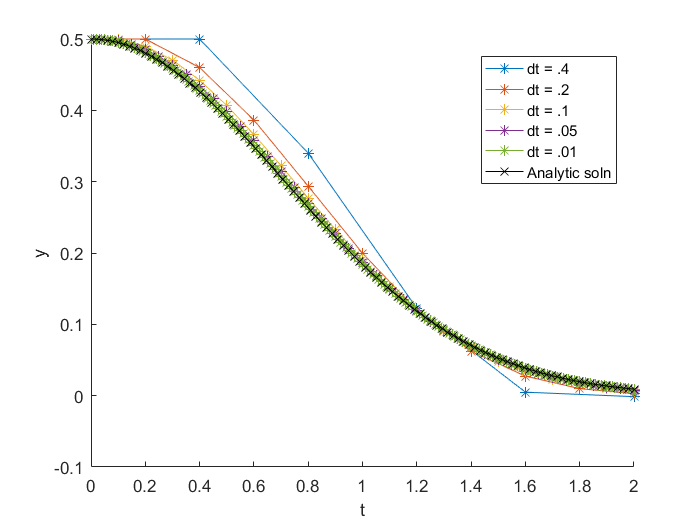
\includegraphics[scale=1]{2_1fig.png}
		\caption{Forward Euler method with various timesteps.}
	\end{figure}
	From this, we see that we get relatively good qualitative agreement very quickly as the step size is decreased. We also see that as $\Delta t \to 0$, the solution converges to the analytic solution.
	\subparagraph{Summary} To derive an explicit scheme for a differential equation, we can write the correspond discrete equation by approximating the derivative(s) using your favorite difference quotient and than evaluating all the other terms at the $n$th time level. You should be able to isolate the $y_{n+1}$ term and write it explicitly in terms of other variables.
	\subsubsection{Improving Euler's Method}
	\subparagraph{Using higher order derivative approximations}
	We used a first order difference quotient in the previous example, but we know that has a first order truncation error. We can approve the accuracy of our scheme by using more accurate approximations of the derivative. For example, let us try using a centered difference quotient. In this case, \eqref{1oIVP} becomes:
	\begin{equation}
		\frac{y_{n+1} - y_{n-1}}{2\Delta t} + f(y_n,t_n) = 0
	\end{equation}
	\begin{equation}
		y_{n+1} = y_{n-1} - f(y_n,t_n)
	\end{equation}
	Wait! We only have one given initial condition, but it seems like to start this scheme we need to know two consecutive values of $y_i$. This is only a minor problem: we can estimate either $y_{-1}$ or $y_{1}$ using Euler's method and then proceed with this scheme.
	\subsection{Implicit Methods}
	The central idea behind explicit methods is to estimate $y_{n+1}$ by performing a taylor expansion around $y_n$. If instead we were to estimate $y_{n+1}$ with a taylor expansion around $y_{n+1}$, we would end up with an \textbf{implicit} method. It is relatively straightforward to convert an explicit method to an implicit method: for every term that does not contain a derivative of $y$, replace the time step $n$ with $n+1$. For instance, to get the simplest implicit method, Implicit Euler,  \ref{1oIVP} becomes
	\begin{equation}
		\frac{y_{n+1} - y_n}{\Delta t} + f(y_{n+1},t_{n+1}) = 0
	\end{equation}
	Notice now that isolating $y_{n+1}$ is more tricky because it also appears in the $f(y_{n+1},t_{n+1})$ term. If the differential equation is non-linear, implicit methods can be rather difficult and computationally expensive to solve depending on the nature of the non-linearity. In the case of linear equations and most ordinary differential equations that engineers encounter, the method is not too different from the normal euler method. At this point, you may well be wondering something along the lines of "Why bother?" It turns out that implicit methods have desirable stability and convergence properties for many differential equations in which achieving reasonable accuracy with an explicit method would require unrealistically small step sizes. These types of differential equations are called "stiff" and can be solved more efficiently using an implicit method and a larger step size.
	
	To fully illustrate the different between explicit and implicit methods, consider the following example.
	\begin{exmp}
		Solve $y'(x) + 4y(x) = 2x\cos(20x)$ on the interval $ 0 \leq x \leq 4 $ given that $y(0) = 2$. Use the implicit Euler method and examine what happens to the convergence of the solution as the step size is varied.
	\end{exmp}
	\textbf{Solution:} Upon inspection of this differential equation, we see that that the cosine term has a frequency of $\frac{2\pi}{20} =  .314159$. Because the period is significantly lower than the length of the interval we are solving $y$ over, we should be cautious and consider that the solution might show significant curvature. Thus, an implicit method is appropriate for solving this problem.
	
	First, we convert our differential equation into a discrete approximation:
	\begin{align*}
			&\frac{y_{n+1} - y_n}{\Delta x} + 4 y_{n+1} = 2 x_{n+1} \cos(20x_{n+1}) \\
			&y_{n+1} - y_n + 4 \Delta x y_{n+1} = 2\Delta x x_{n+1} \cos(20x_{n+1}) \\
			&(1 + 4\Delta x) y_{n+1} = y_n + 2\Delta x x_{n+1} \cos(20x_{n+1})\\
			&y_{n+1} = \frac{y_n + 2\Delta x x_{n+1} \cos(20x_{n+1})}{1 + 4\Delta x}
	\end{align*}
	Since we are given $y_0 = 2$, we now have a straightforward way of calculating this scheme.
		\begin{center}
		\begin{figure}[H]
			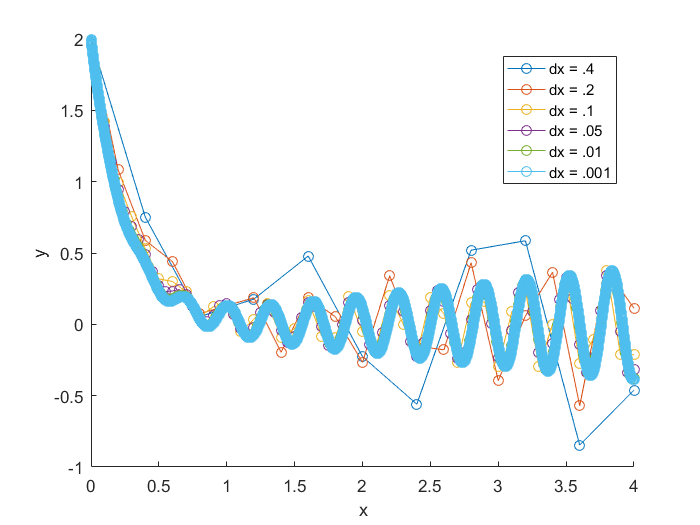
\includegraphics[scale=.75]{ex3_fig.png} 
			\caption{Implicit Euler with various timesteps.}
			\label{fig:implic1}
		\end{figure}
	\end{center}
	\subsection{Predictor-Corrector Methods}
	\subsubsection{Modified Euler/Heun Method}
	Numerical methods for differential equations are a lot like ice cream. There are so many options to choose from and choosing a flavor can be very difficult. However, humans have a knack for ingenuity and discovered long ago that ice cream can be mixed so that I can get half chocolate and half vanilla or any combination that I want. In much the same way, the choice of a numerical scheme can seem overwhelming. Just like with ice cream, it turns out that combining implicit and explicit methods works out well. These schemes are called "Predictor-Corrector Methods". They combine the the best properties of both explicit and implicit methods and are very popular in practice.
	
	The basic concept behind this method is to make a prediction using an explicit scheme expanded about $y_i$ to "predict" a later point such as $y_{i+.5}$ or $y_{i+1}$ Let's call this prediction $y^*$. The next step is to "correct" the estimate of $y_{i+1}$ using a weighted average of explicit methods expanded about $y_i$ and $y^*$. For higher order methods of this type, there can be more than one prediction step.

	If that description sounds abstract, that is okay. Formally stating this algorithm should hopefully illustrate what is going on. The simplest predictor-corrector method is called the "modified Euler method" or "Heun's" method. Suppose we are attempting to solve
	\begin{equation}
		\frac{\text{d}y}{\text{d}x} = f(y,x) , \qquad f(x=x_0) = a \label{ModEulerDE}
	\end{equation}
	with $a$ being a constant. The first step is to use Euler's method to "predict" $y_{n+1}$:
	\begin{equation}
		y^*_{n+1} = y_{n} + \Delta x f(y_n,x_n)
	\end{equation}
	The second step is to "correct" the estimate for $y_{n+1}$ using the prediction:
	\begin{equation}
		y_{n+1} = y_n +  \frac{\Delta x}{2} \left(f(y^*_{n+1},x_{n+1}) + f(y_n,x_n)\right)
	\end{equation}
	Although we are doing more computations with this algorithm than an implicit or euler, it turns out that the increase in the number of computations corresponds to a negligible increase in computation time. If you are familar with complexity analysis, this means that these methods have the same run time as the simpler implicit or explicit methods. To illustrate the utility of predictor corrector methods, let us consider applying this scheme to a solution with significant curvature.
	
	\begin{exmp}
	Solve $y'(x) + (y(x))^3 = 2x\cos^2(25x)$ on the interval $ 0 \leq x \leq 10 $ given that $y(0) = 2$. Use the modified Euler method and examine how the convergence depends on $\Delta x$.
	\end{exmp}
	\textbf{Solution:} The first step consists of a prediction:
	\begin{equation*}
		y^*_{n+1} = y_n + \Delta x \left(2x_n \cos^2(25x_n) - (y_n)^3\right)
	\end{equation*}
	The second step is the correction:
		\begin{equation*}
			y_{n+1} = y_n + \frac{\Delta x}{2} \left(2x_{n+1}\cos^2(25x_{n+1}) - (y^*_{n+1})^3 + 2x_n \cos^2(25x_n) - (y_n)^3\right)
		\end{equation*}
	From which we can now code up the scheme. As an illustration of how one might go about coding this up, a sample Matlab code is given.
		\lstinputlisting{ex_4.m}
		\begin{center}
		\begin{figure}[H]
			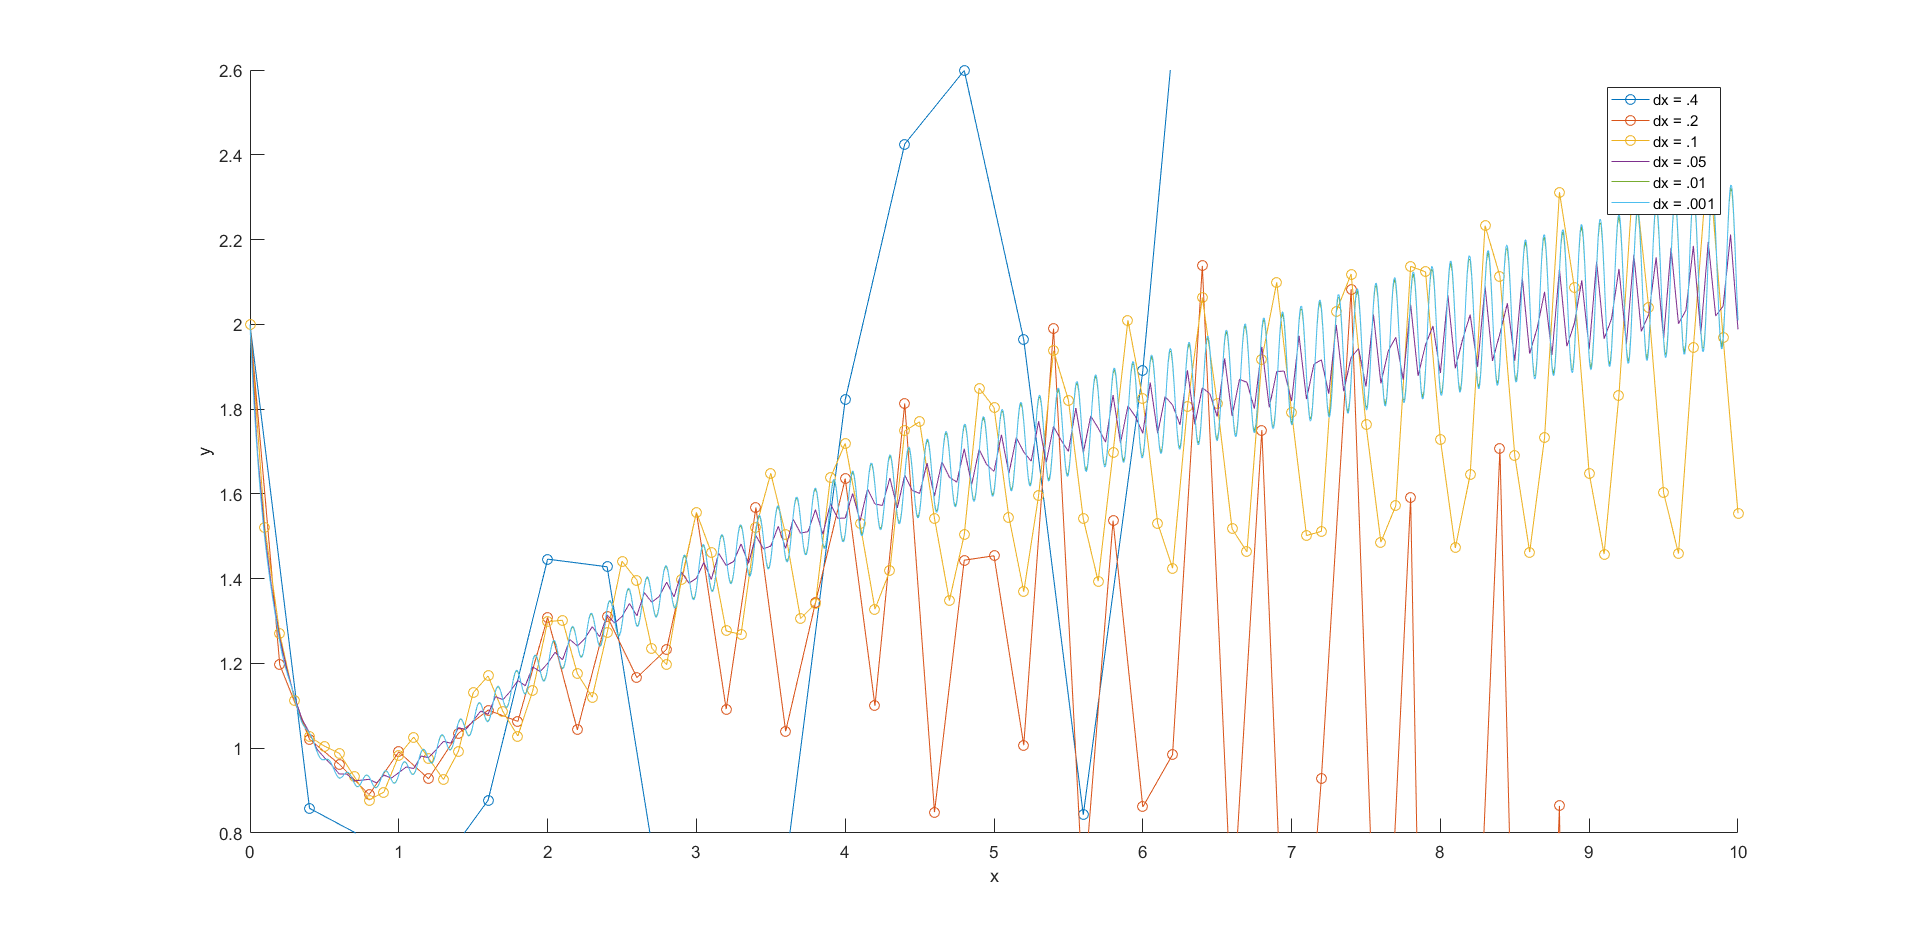
\includegraphics[scale=.35]{ex4_1_fig.png} 
			\caption{Heun's method with various step sizes. For functions with a lot of curvature, larger step sizes are unstable.}
			\label{fig:Heun1_1}
		\end{figure}
		\begin{figure}[H]
		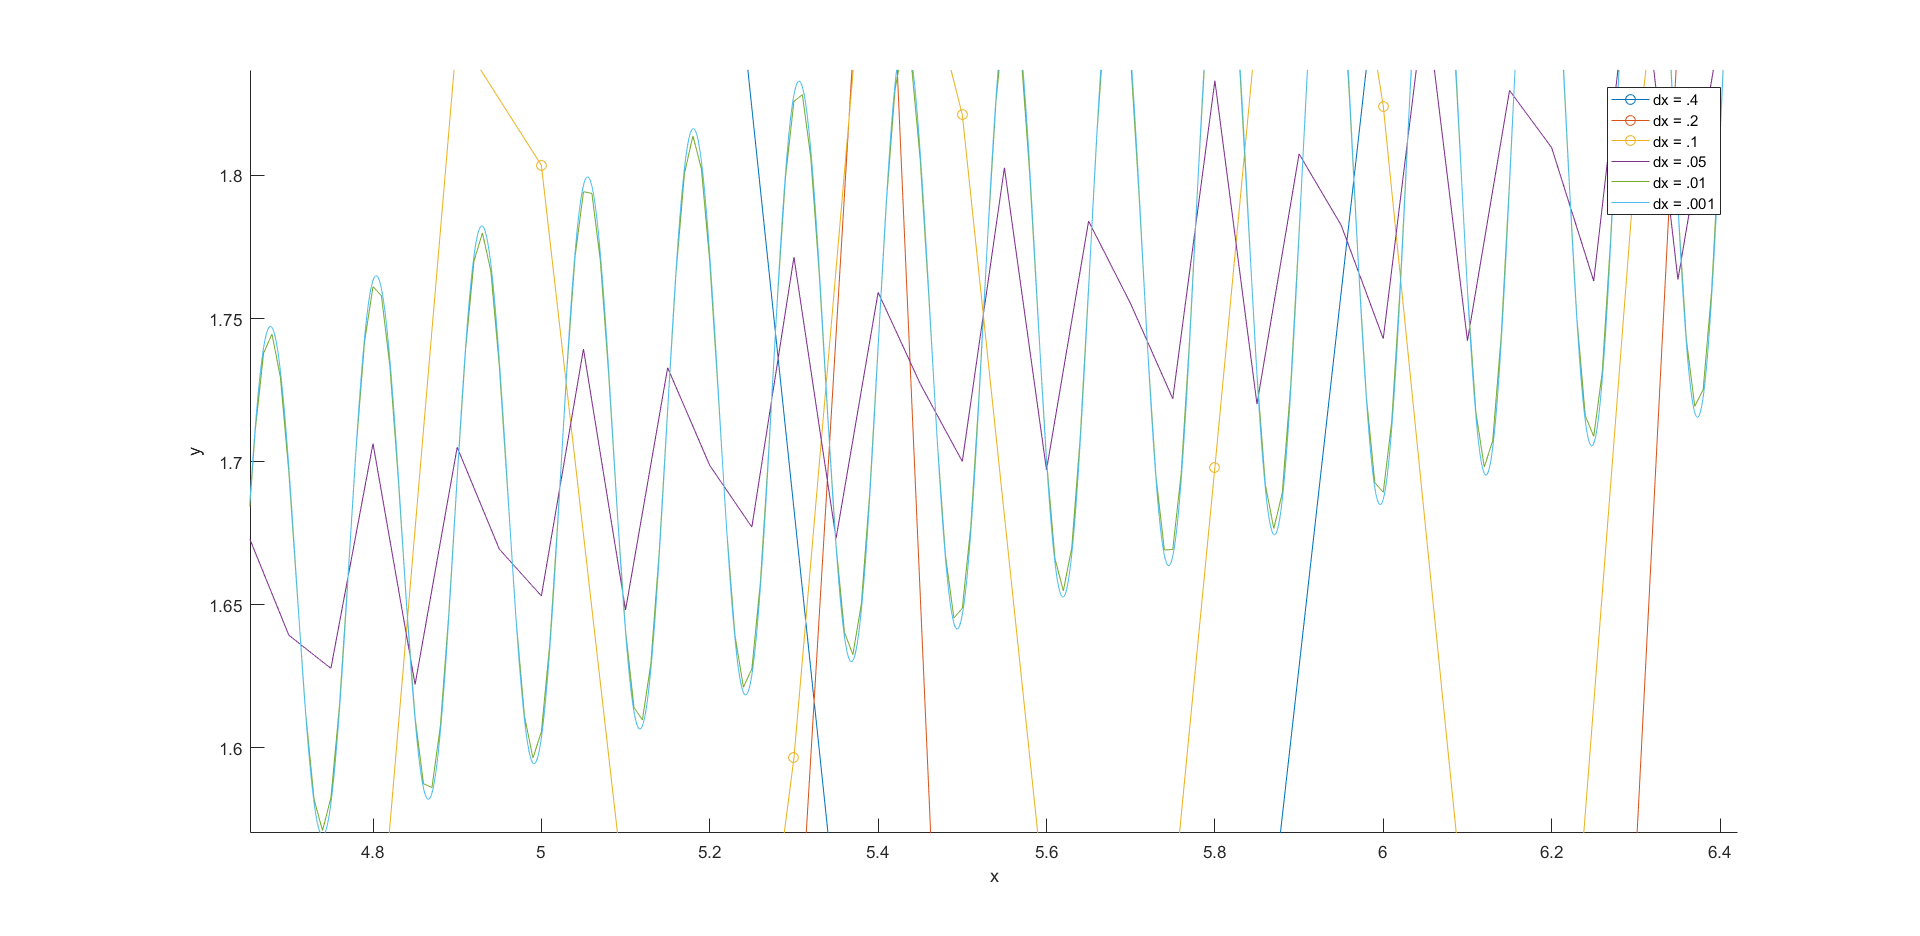
\includegraphics[scale=.3]{ex4_2_fig.png} 
		\caption{Zoomed-in section of previous plot}
		\label{fig:Heun1_2}
	\end{figure}
%%% This file was created by matlab2tikz.
%
%The latest updates can be retrieved from
%  http://www.mathworks.com/matlabcentral/fileexchange/22022-matlab2tikz-matlab2tikz
%where you can also make suggestions and rate matlab2tikz.
%
\definecolor{mycolor1}{rgb}{0.00000,0.44700,0.74100}%
\definecolor{mycolor2}{rgb}{0.85000,0.32500,0.09800}%
\definecolor{mycolor3}{rgb}{0.92900,0.69400,0.12500}%
\definecolor{mycolor4}{rgb}{0.49400,0.18400,0.55600}%
\definecolor{mycolor5}{rgb}{0.46600,0.67400,0.18800}%
\definecolor{mycolor6}{rgb}{0.30100,0.74500,0.93300}%
%
\begin{tikzpicture}

\begin{axis}[%
width=5.431in,
height=4.849in,
at={(0.911in,0.654in)},
scale only axis,
unbounded coords=jump,
xmin=0,
xmax=10,
xlabel style={font=\color{white!15!black}},
xlabel={x},
ymin=0.8,
ymax=2.6,
ylabel style={font=\color{white!15!black}},
ylabel={y},
axis background/.style={fill=white},
axis x line*=bottom,
axis y line*=left,
legend style={at={(0.1,0.712)}, anchor=south west, legend cell align=left, align=left, draw=white!15!black}
]
\addplot [color=mycolor1, mark=o, mark options={solid, mycolor1}]
  table[row sep=crcr]{%
0	2\\
0.4	0.858246564945071\\
0.8	0.78311365980991\\
1.2	0.683878895562798\\
1.6	0.877229826528619\\
2	1.4460818165795\\
2.4	1.42802541321662\\
2.76983677099147	0.62\\
nan	nan\\
3.6	0.722133816366612\\
4	1.82172394704788\\
4.4	2.42534097196421\\
4.8	2.59884739475535\\
5.2	1.96363116198469\\
5.6	0.843156378969621\\
6	1.88997499450146\\
6.2320066079632	2.78\\
};
\addlegendentry{dx = .4}

\addplot [color=mycolor2, mark=o, mark options={solid, mycolor2}]
  table[row sep=crcr]{%
0	2\\
0.199999999999999	1.19681856941847\\
0.4	1.02123739107689\\
0.6	0.962218615002868\\
0.800000000000001	0.890511646406459\\
1	0.991340697135994\\
1.2	0.927826055316837\\
1.4	1.03496405177365\\
1.6	1.08999088359159\\
1.8	1.06330726930737\\
2	1.30828913910157\\
2.2	1.04331030775603\\
2.4	1.31090876849362\\
2.6	1.16672428658767\\
2.8	1.23351295993866\\
3	1.55675895949679\\
3.2	1.09245618408022\\
3.4	1.56796511510105\\
3.6	1.04009420686076\\
3.8	1.34270912180225\\
4	1.63583395634978\\
4.2	1.10013607212014\\
4.4	1.81324125758257\\
4.6	0.849188528961495\\
4.8	1.44360004653767\\
5	1.45399070984497\\
5.2	1.00723890173519\\
5.4	1.9897302115317\\
5.6	0.644799549853619\\
5.8	1.53674382828072\\
6	0.861436452426465\\
6.2	0.984951878460494\\
6.4	2.1378653942742\\
6.59557367611227	0.619999999999999\\
nan	nan\\
6.60589749290842	0.619999999999999\\
6.8	1.75065411464787\\
6.93040962994387	0.619999999999999\\
nan	nan\\
7.13242766062503	0.619999999999999\\
7.2	0.927864418660823\\
7.4	2.08311224470194\\
7.5475746706826	0.619999999999999\\
nan	nan\\
7.66970600221076	0.619999999999999\\
7.8	1.59154120212039\\
7.85069237826221	0.619999999999999\\
nan	nan\\
8.25299697639439	0.620000000000001\\
8.25299697639439	0.619999999999999\\
nan	nan\\
8.27111409642103	0.619999999999999\\
8.4	1.70639065320679\\
8.47663736248116	0.619999999999999\\
nan	nan\\
8.77552344547655	0.620000000000001\\
8.8	0.86386207512499\\
8.8086625991775	0.620000000000001\\
};
\addlegendentry{dx = .2}

\addplot [color=mycolor3, mark=o, mark options={solid, mycolor3}]
  table[row sep=crcr]{%
0	2\\
0.0999999999999996	1.52001831092732\\
0.199999999999999	1.26995006327609\\
0.300000000000001	1.11178696676278\\
0.4	1.02755457404172\\
0.5	1.00485075915357\\
0.6	0.98808362822354\\
0.699999999999999	0.933490841467369\\
0.800000000000001	0.877832115009957\\
0.9	0.896670493132437\\
1	0.983017516674444\\
1.1	1.02620691303091\\
1.2	0.976516891369783\\
1.3	0.926110419591211\\
1.4	0.992283577666809\\
1.5	1.13103700088694\\
1.6	1.17045460787423\\
1.7	1.08624785485586\\
1.8	1.02882584925338\\
1.9	1.13546894602186\\
2	1.29844368965527\\
2.1	1.30185746007728\\
2.2	1.17587028331026\\
2.3	1.12016508603714\\
2.4	1.27207743508115\\
2.5	1.44101823291267\\
2.6	1.39662164136284\\
2.7	1.23618058739903\\
2.8	1.19695617195783\\
2.9	1.39900326663908\\
3	1.55663879104024\\
3.1	1.46141302503658\\
3.2	1.2767822119946\\
3.3	1.2683017837033\\
3.4	1.52056393992242\\
3.5	1.64859603945649\\
3.6	1.50398636222985\\
3.7	1.30565511408822\\
3.8	1.34078520009485\\
3.9	1.63768759141215\\
4	1.71909865784286\\
4.1	1.52968082981825\\
4.2	1.32815448563601\\
4.3	1.41832784925049\\
4.4	1.74851740517683\\
4.5	1.77009324415587\\
4.6	1.54245022817021\\
4.7	1.34827715900892\\
4.8	1.5032139424112\\
4.9	1.84976620383917\\
5	1.80354742519517\\
5.1	1.54542969699215\\
5.2	1.36928993539317\\
5.3	1.59647745998658\\
5.4	1.93776803677925\\
5.5	1.82115090078574\\
5.6	1.54106773596684\\
5.7	1.39393614334117\\
5.8	1.69792809021412\\
5.9	2.00944808653288\\
6	1.82420596447603\\
6.1	1.53124126979001\\
6.2	1.42453410041673\\
6.3	1.80608450855098\\
6.4	2.06316044356748\\
6.5	1.81404556851033\\
6.6	1.51756794379954\\
6.7	1.46312695413363\\
6.8	1.91816203222378\\
6.9	2.09906916346963\\
7	1.79267380751564\\
7.1	1.50180228806902\\
7.2	1.51164550382327\\
7.3	2.03014597531307\\
7.4	2.1187075487195\\
7.5	1.76294693108927\\
7.6	1.4860118920405\\
7.7	1.57191557179441\\
7.8	2.13695126195602\\
7.9	2.1236677938223\\
8	1.7278797243637\\
8.1	1.47235479183112\\
8.2	1.64539074647066\\
8.3	2.23276564378946\\
8.4	2.11397437877084\\
8.5	1.6894482809058\\
8.6	1.46261252907408\\
8.7	1.73268995480182\\
8.8	2.3117731783642\\
8.9	2.08724026512086\\
9	1.64794428518572\\
9.1	1.45792669197202\\
9.2	1.83322477359843\\
9.3	2.3693503681138\\
9.4	2.03964153460595\\
9.5	1.60276920493782\\
9.6	1.45917594832313\\
9.7	1.94520424534149\\
9.8	2.40346778288493\\
9.9	1.96874494014904\\
10	1.55430417594491\\
};
\addlegendentry{dx = .1}

\addplot [color=mycolor4]
  table[row sep=crcr]{%
0	2\\
0.0500000000000007	1.69784857048057\\
0.0999999999999996	1.50215801154928\\
0.15	1.36564629328388\\
0.199999999999999	1.2591870152454\\
0.25	1.18344476322111\\
0.300000000000001	1.12064938342251\\
0.35	1.06867440452683\\
0.4	1.0356750578804\\
0.449999999999999	0.997781892464484\\
0.5	0.977763512717146\\
0.550000000000001	0.959616915568658\\
0.6	0.939083307425879\\
0.65	0.93928512445795\\
0.699999999999999	0.922969191183816\\
0.800000000000001	0.926627180020853\\
0.85	0.918290445820148\\
0.9	0.936539891167492\\
0.949999999999999	0.929580110653404\\
1.05	0.955851419566176\\
1.1	0.95194435807826\\
1.15	0.981460993085978\\
1.2	0.977767450670843\\
1.25	0.996258791884266\\
1.3	1.01606402359025\\
1.35	1.01190841102407\\
1.4	1.04853611812053\\
1.45	1.04419898109193\\
1.5	1.06465528072781\\
1.55	1.08781123388063\\
1.6	1.08042320244549\\
1.65	1.1216668279951\\
1.7	1.11435839546767\\
1.75	1.13463806319515\\
1.8	1.15959999403422\\
1.85	1.14736386815598\\
1.9	1.19206389445137\\
1.95	1.18077706077089\\
2	1.1998443275998\\
2.05	1.22626433095002\\
2.1	1.2085332159566\\
2.15	1.25640339065316\\
2.2	1.24099400038368\\
2.25	1.25844580811013\\
2.3	1.28665976760136\\
2.35	1.26328279520449\\
2.4	1.31442785889492\\
2.45	1.29515171521608\\
2.5	1.31082181110141\\
2.55	1.34143349392764\\
2.6	1.31241570860122\\
2.65	1.36701921924706\\
2.7	1.3442482846989\\
2.75	1.35799484599415\\
2.8	1.39165979853736\\
2.85	1.3570027778281\\
2.9	1.41519442933731\\
2.95	1.38930656913682\\
3	1.40094080414966\\
3.05	1.43829338108353\\
3.1	1.39795032508806\\
3.15	1.4597740673091\\
3.2	1.43113545860518\\
3.25	1.44041524996439\\
3.3	1.48205781702958\\
3.35	1.43593446505977\\
3.4	1.50135292913561\\
3.45	1.47033195431778\\
3.5	1.47697366278035\\
3.55	1.52348140396313\\
3.6	1.47144748148784\\
3.65	1.54035322052362\\
3.7	1.50733886244206\\
3.75	1.51102937250187\\
3.8	1.56295400795903\\
3.85	1.50485375099666\\
3.9	1.57707883570885\\
3.95	1.54249600196027\\
4	1.54290105058783\\
4.05	1.60077035977797\\
4.1	1.53643051784356\\
4.15	1.61175374175645\\
4.2	1.57607483739218\\
4.25	1.57284397245496\\
4.3	1.63715797045365\\
4.35	1.56639424003496\\
4.4	1.64454683718865\\
4.45	1.60830031166233\\
4.5	1.6010694591004\\
4.55	1.67229454306013\\
4.6	1.59491750700157\\
4.65	1.67558816218826\\
4.7	1.63936461603861\\
4.75	1.62775699404474\\
4.8	1.70631907123119\\
4.85	1.62214037696679\\
4.9	1.70497994762651\\
4.95	1.66943606605641\\
5	1.65306191558694\\
5.05	1.73933921844938\\
5.1	1.64817843287402\\
5.15	1.73280454490329\\
5.2	1.6986649228222\\
5.25	1.67712036476884\\
5.3	1.77143646106662\\
5.35	1.67312884425391\\
5.4	1.75913037818496\\
5.45	1.72718721257012\\
5.5	1.70005246613028\\
5.55	1.80266984883331\\
5.6	1.69707515690036\\
5.65	1.78401656433666\\
5.7	1.75512717239952\\
5.75	1.72196433956614\\
5.8	1.83307889477071\\
5.85	1.72009122268923\\
5.9	1.80751657538228\\
5.95	1.78259872039972\\
6	1.74294933535519\\
6.05	1.86268591592937\\
6.1	1.74224450725834\\
6.15	1.82968116631707\\
6.2	1.80970621933737\\
6.25	1.76308876696325\\
6.3	1.89149803558233\\
6.35	1.7635989107006\\
6.4	1.85056070245881\\
6.45	1.83654472686749\\
6.5	1.7824523452371\\
6.55	1.91950898931239\\
6.6	1.78421717452946\\
6.65	1.87020696764874\\
6.7	1.86319987777319\\
6.75	1.80109847160225\\
6.8	1.94670083357551\\
6.85	1.80416291084022\\
6.9	1.88867450318073\\
6.95	1.88974751252494\\
7	1.81907451543312\\
7.05	1.97304562553265\\
7.1	1.82350226801058\\
7.15	1.90602150945925\\
7.2	1.9162531446731\\
7.25	1.83641717550636\\
7.3	1.99850712142563\\
7.35	1.84230523626119\\
7.4	1.9223103334242\\
7.45	1.94277134340138\\
7.5	1.85315300369234\\
7.55	2.02304252403037\\
7.6	1.86064659257301\\
7.65	1.9376075618083\\
7.7	1.96934509473794\\
7.75	1.86929914865684\\
7.8	2.04660429560878\\
7.85	1.87860648545201\\
7.9	1.95198374134771\\
7.95	1.99600519412838\\
8	1.88486435718867\\
8.05	2.06914204002711\\
8.1	1.8962706640206\\
8.15	1.96551275076402\\
8.2	2.02276971355405\\
8.25	1.89985025038229\\
8.3	2.09060444566215\\
8.35	1.91373036144024\\
8.4	1.97827085467131\\
8.45	2.04964357772014\\
8.5	1.91425287135698\\
8.55	2.11094126919865\\
8.6	1.93108184857876\\
8.65	1.99033547581953\\
8.7	2.07661827588287\\
8.75	1.92806448097335\\
8.8	2.1301053296213\\
8.85	1.94842567927699\\
8.9	2.00178372877711\\
8.95	2.10367172866367\\
9	1.94127555892812\\
9.05	2.14805447207503\\
9.1	1.96586565301767\\
9.15	2.01269076499298\\
9.2	2.13076832288809\\
9.25	1.95387695070194\\
9.3	2.16475345341793\\
9.35	1.98350752407549\\
9.4	2.0231279860199\\
9.45	2.15785912235762\\
9.5	1.96586208723445\\
9.55	2.18017569586988\\
9.6	2.0014574884754\\
9.65	2.03316118847756\\
9.7	2.184882258808\\
9.75	1.97722919499431\\
9.8	2.19430485273229\\
9.85	2.01982048172135\\
9.9	2.04284871103299\\
9.95	2.21176350536545\\
10	1.9879834101975\\
};
\addlegendentry{dx = .05}

\addplot [color=mycolor5]
  table[row sep=crcr]{%
0	2\\
0.00999999999999979	1.92470443912809\\
0.0199999999999996	1.85745925827586\\
0.0299999999999994	1.79687726192308\\
0.0399999999999991	1.74184317953692\\
0.0500000000000007	1.69148472480047\\
0.0600000000000005	1.64515611577033\\
0.0700000000000003	1.60241355863365\\
0.0800000000000001	1.56297149272857\\
0.0899999999999999	1.52663918892242\\
0.0999999999999996	1.49324729557086\\
0.109999999999999	1.46258058215604\\
0.119999999999999	1.43433452343173\\
0.130000000000001	1.40810889885174\\
0.15	1.35987987675692\\
0.17	1.31476951455759\\
0.19	1.27201644355361\\
0.199999999999999	1.25208986110478\\
0.210000000000001	1.23361916873134\\
0.220000000000001	1.21689895896346\\
0.23	1.20203591642632\\
0.24	1.1888852264712\\
0.26	1.16595291182575\\
0.279999999999999	1.14351359929791\\
0.300000000000001	1.11837179506704\\
0.32	1.09187443008154\\
0.33	1.07964365934434\\
0.34	1.06898296372474\\
0.35	1.06029929702247\\
0.359999999999999	1.0536297496287\\
0.369999999999999	1.0486044478435\\
0.390000000000001	1.04045973798462\\
0.4	1.03558306780351\\
0.41	1.02926778579059\\
0.42	1.02131298860851\\
0.44	1.00203943040666\\
0.449999999999999	0.992413290200423\\
0.460000000000001	0.984133433551634\\
0.470000000000001	0.977987374135047\\
0.48	0.974326462419276\\
0.49	0.972955076862469\\
0.52	0.973802541480758\\
0.529999999999999	0.972045235082206\\
0.540000000000001	0.96799729306845\\
0.550000000000001	0.961695623966305\\
0.58	0.937868925512367\\
0.59	0.932390956331448\\
0.6	0.929754448047307\\
0.609999999999999	0.930102020466196\\
0.619999999999999	0.932876125929894\\
0.640000000000001	0.940809081844467\\
0.65	0.943075958145776\\
0.66	0.942699233087655\\
0.67	0.939307671258293\\
0.68	0.933304280451617\\
0.699999999999999	0.918296318531839\\
0.710000000000001	0.912441802823734\\
0.720000000000001	0.909505989512173\\
0.73	0.910112927165134\\
0.74	0.914052013299598\\
0.75	0.920304711309118\\
0.76	0.927274934413362\\
0.77	0.9331715441624\\
0.779999999999999	0.936450390885785\\
0.790000000000001	0.936205355765681\\
0.800000000000001	0.932408725961366\\
0.810000000000001	0.925938089726007\\
0.82	0.918379492387558\\
0.83	0.911651216248497\\
0.84	0.907536519526769\\
0.85	0.907237533308724\\
0.859999999999999	0.911060792462706\\
0.869999999999999	0.918316665753173\\
0.890000000000001	0.936477716333577\\
0.9	0.943333934033962\\
0.91	0.946523221052512\\
0.92	0.945431864493415\\
0.93	0.940512302609402\\
0.949999999999999	0.925537127279798\\
0.960000000000001	0.919760740958999\\
0.970000000000001	0.917673606543749\\
0.98	0.920229071915628\\
0.99	0.92726521045811\\
1	0.937518341935441\\
1.01	0.948912445270022\\
1.02	0.959059313957967\\
1.03	0.965847683815625\\
1.04	0.96797355949951\\
1.05	0.965277208145142\\
1.06	0.958800970422297\\
1.07	0.950551596643384\\
1.08	0.943022453935345\\
1.09	0.938588234868449\\
1.1	0.938916444762837\\
1.11	0.944539574155129\\
1.12	0.954697965719879\\
1.14	0.980374373454753\\
1.15	0.990690733529458\\
1.16	0.996421589568916\\
1.17	0.996650853504281\\
1.18	0.991816652292339\\
1.19	0.983621508490613\\
1.2	0.974631472266841\\
1.21	0.967658978309522\\
1.22	0.96507526009797\\
1.23	0.968217097296796\\
1.24	0.97703509221086\\
1.25	0.990077574149144\\
1.26	1.00482440350382\\
1.27	1.01829602303644\\
1.28	1.02778888219734\\
1.29	1.03155178974627\\
1.3	1.02923149442661\\
1.31	1.02197564084167\\
1.33	1.00285919864457\\
1.34	0.997028851643773\\
1.35	0.996851381394688\\
1.36	1.00314517084238\\
1.37	1.01514361147429\\
1.39	1.04658478204316\\
1.4	1.05969031172476\\
1.41	1.06738978508755\\
1.42	1.06840934417439\\
1.43	1.06311099199185\\
1.44	1.05341881519266\\
1.45	1.04236330859733\\
1.46	1.03335301470741\\
1.47	1.0293449041445\\
1.48	1.03211019118577\\
1.49	1.04177564415876\\
1.5	1.0567615558236\\
1.51	1.07414448248741\\
1.52	1.09036508274309\\
1.53	1.10210766784462\\
1.54	1.10712824389027\\
1.55	1.1048199676861\\
1.56	1.09637520143328\\
1.58	1.07280209902424\\
1.59	1.06485165405108\\
1.6	1.0633753658605\\
1.61	1.06953636848824\\
1.62	1.0826261665542\\
1.64	1.11869202825308\\
1.65	1.13422321675527\\
1.66	1.14363251839254\\
1.67	1.14523414420151\\
1.68	1.13925096215278\\
1.69	1.12777118557821\\
1.7	1.11425112067935\\
1.71	1.10268514350399\\
1.72	1.09663749830772\\
1.73	1.0983628734495\\
1.74	1.1082289288429\\
1.75	1.12459176315008\\
1.77	1.1628444094253\\
1.78	1.17666843160505\\
1.79	1.18286222847999\\
1.8	1.18050438279217\\
1.81	1.17076826707214\\
1.83	1.14222718635975\\
1.84	1.13172298139738\\
1.85	1.1284315001899\\
1.86	1.13391935116299\\
1.87	1.14760414260731\\
1.88	1.16686171747763\\
1.89	1.18764846389855\\
1.9	1.20549406499579\\
1.91	1.2166144896234\\
1.92	1.21885783741238\\
1.93	1.21224239585758\\
1.94	1.19895881089934\\
1.95	1.18284528151267\\
1.96	1.16846645035371\\
1.97	1.16001130371849\\
1.98	1.16026538263152\\
1.99	1.169903382205\\
2	1.18728530325829\\
2.02	1.22986327091093\\
2.03	1.24581372774026\\
2.04	1.25331719762643\\
2.05	1.25107554019687\\
2.06	1.24017610734509\\
2.08	1.20660626112439\\
2.09	1.19332433703\\
2.1	1.18789570949262\\
2.11	1.19234867550954\\
2.12	1.20629755171703\\
2.13	1.22699632493535\\
2.14	1.2499869821386\\
2.15	1.27019468538869\\
2.16	1.28319317005624\\
2.17	1.28631084421598\\
2.18	1.27929410166812\\
2.19	1.26437053101058\\
2.2	1.24571126745013\\
2.21	1.22843025640509\\
2.22	1.21735409798956\\
2.23	1.2158440349899\\
2.24	1.22494840372544\\
2.25	1.24310274795498\\
2.27	1.28989205933644\\
2.28	1.30812366762881\\
2.29	1.31719041621194\\
2.3	1.31535527890428\\
2.31	1.30355022224712\\
2.32	1.28514757133791\\
2.33	1.26514772811449\\
2.34	1.24898069943978\\
2.35	1.24119555996135\\
2.36	1.24433868242568\\
2.37	1.25829306735034\\
2.38	1.28025991836373\\
2.39	1.30541472057266\\
2.4	1.32809247417085\\
2.41	1.3432026851057\\
2.42	1.34750248810111\\
2.43	1.34039852397684\\
2.44	1.32408704378429\\
2.46	1.28282997031689\\
2.47	1.26899277235722\\
2.48	1.26548496363979\\
2.49	1.27379410676012\\
2.5	1.29250525785741\\
2.52	1.34343690143552\\
2.53	1.36413047633509\\
2.54	1.37504845072545\\
2.55	1.37395412117908\\
2.56	1.36155355774853\\
2.57	1.34131497195306\\
2.58	1.31862962950907\\
2.59	1.29952186048354\\
2.6	1.28920146416476\\
2.61	1.29078604386492\\
2.62	1.30449923774147\\
2.63	1.32756190813624\\
2.64	1.35483673524467\\
2.65	1.38008940739008\\
2.66	1.39754863157684\\
2.67	1.40335190998442\\
2.68	1.39649889969377\\
2.69	1.37908435317953\\
2.71	1.33271534009928\\
2.72	1.31600638610646\\
2.73	1.31028452871304\\
2.74	1.31753981390522\\
2.75	1.33658195497101\\
2.76	1.36327847622799\\
2.77	1.39154669811572\\
2.78	1.41486579085229\\
2.79	1.42791453854699\\
2.8	1.42789816309998\\
2.81	1.41522607962123\\
2.82	1.39339540686781\\
2.83	1.36813969182264\\
2.84	1.34605854055587\\
2.85	1.33303851011191\\
2.86	1.33281731466618\\
2.87	1.34603004232474\\
2.88	1.36999215371157\\
2.9	1.42721543803173\\
2.91	1.44723790568091\\
2.92	1.45485359307351\\
2.93	1.44858936806127\\
2.94	1.43036710080931\\
2.96	1.37912812334771\\
2.97	1.35945143383343\\
2.98	1.35130364291978\\
2.99	1.35723726910937\\
3	1.37636208687405\\
3.01	1.40450040036066\\
3.02	1.43518342676987\\
3.03	1.46125975023864\\
3.04	1.47669583582045\\
3.05	1.47808348919192\\
3.06	1.46546507606991\\
3.07	1.44229740243059\\
3.08	1.41460319703546\\
3.09	1.38953221519855\\
3.1	1.37365743858116\\
3.11	1.37138061346386\\
3.12	1.38381711111029\\
3.13	1.40845369781176\\
3.15	1.4703019802905\\
3.16	1.49307202466058\\
3.17	1.50278980279774\\
3.18	1.49744555418923\\
3.19	1.47871614886695\\
3.2	1.45153090572012\\
3.21	1.42288025232092\\
3.22	1.40015394707961\\
3.23	1.38937327500959\\
3.24	1.39370927012682\\
3.25	1.41264668416373\\
3.26	1.44203712024328\\
3.27	1.4750796049984\\
3.28	1.5040110265881\\
3.29	1.52206555833232\\
3.3	1.5251697786238\\
3.31	1.51292943413807\\
3.32	1.48868997675185\\
3.33	1.45870603206566\\
3.34	1.43064644032208\\
3.35	1.41177375415868\\
3.36	1.40719224033185\\
3.37	1.41856372766041\\
3.38	1.44362410244184\\
3.4	1.50995760831694\\
3.41	1.53562965952982\\
3.42	1.54771956660978\\
3.43	1.54361950234602\\
3.44	1.52468890103961\\
3.45	1.49588598910409\\
3.46	1.46456326456984\\
3.47	1.43872284066387\\
3.48	1.4251114831953\\
3.49	1.42757029245337\\
3.5	1.44603274955734\\
3.51	1.47645697478964\\
3.52	1.51176947898231\\
3.53	1.54362132152932\\
3.54	1.56450056392299\\
3.55	1.56962068884196\\
3.56	1.5580824887342\\
3.57	1.53304759319398\\
3.59	1.46991506418432\\
3.6	1.44791726932022\\
3.61	1.44078749574657\\
3.62	1.45079693323152\\
3.63	1.47600885810012\\
3.65	1.54662395630228\\
3.66	1.5753236119602\\
3.67	1.59003656462841\\
3.68	1.58749829112021\\
3.69	1.56867843295609\\
3.7	1.53849433188669\\
3.71	1.50460786801317\\
3.72	1.47560949973526\\
3.73	1.4589829997468\\
3.74	1.45928611166196\\
3.75	1.47697297803886\\
3.76	1.50818755942336\\
3.77	1.54564897542149\\
3.78	1.58045534622\\
3.79	1.60434125939356\\
3.8	1.61176357848965\\
3.81	1.60125144294619\\
3.82	1.57570915410176\\
3.84	1.50772007163065\\
3.85	1.48248932992057\\
3.86	1.47257734177618\\
3.87	1.4809237106953\\
3.88	1.50599716370326\\
3.89	1.54207761706743\\
3.9	1.58063070017421\\
3.91	1.6124553103742\\
3.92	1.63002306370621\\
3.93	1.62935733129518\\
3.94	1.61096607853107\\
3.95	1.57965387055299\\
3.96	1.54333490273838\\
3.97	1.51115789435599\\
3.98	1.49134854889294\\
3.99	1.48922242018977\\
4	1.5058237749173\\
4.01	1.53756321066019\\
4.03	1.61478720442661\\
4.04	1.64183734811644\\
4.05	1.65183456087473\\
4.06	1.64267167395389\\
4.07	1.61692150566052\\
4.09	1.54435337531989\\
4.1	1.51580377287219\\
4.11	1.50288861161861\\
4.12	1.50927055959705\\
4.13	1.53390096581943\\
4.14	1.57116843429041\\
4.15	1.61223360191942\\
4.16	1.64725229764297\\
4.17	1.66788679175416\\
4.18	1.66939657831598\\
4.19	1.65175693551093\\
4.2	1.61958604292909\\
4.21	1.58098931270524\\
4.22	1.54563777591552\\
4.23	1.5224973288245\\
4.24	1.51767670117615\\
4.25	1.53287663850022\\
4.26	1.56485598069525\\
4.28	1.6468305602626\\
4.29	1.67717752167487\\
4.3	1.69000766720684\\
4.31	1.6825153231898\\
4.32	1.65686741074562\\
4.33	1.61960210679552\\
4.34	1.58004345439982\\
4.35	1.54811291780452\\
4.36	1.53198943751499\\
4.37	1.53610847781443\\
4.38	1.55997960373521\\
4.39	1.59818241399347\\
4.4	1.64163859755064\\
4.41	1.67989199079305\\
4.42	1.70378431177778\\
4.43	1.70776347106207\\
4.44	1.6912023236542\\
4.45	1.65845771943425\\
4.46	1.61776151330284\\
4.47	1.57926547805368\\
4.48	1.55266729664723\\
4.49	1.54489809858318\\
4.5	1.55837773585625\\
4.51	1.59029501260311\\
4.53	1.67675765123682\\
4.54	1.71050822135332\\
4.55	1.72641329993237\\
4.56	1.72090939272628\\
4.57	1.69568323999817\\
4.58	1.65716833445198\\
4.59	1.61497211057375\\
4.6	1.57962385659594\\
4.61	1.56010514597011\\
4.62	1.56166857639466\\
4.63	1.58445525918911\\
4.64	1.6233199729252\\
4.65	1.66901706404167\\
4.66	1.71051681364948\\
4.67	1.73783595913562\\
4.68	1.74456761894423\\
4.69	1.72941417186121\\
4.7	1.69639523849731\\
4.72	1.61221714098572\\
4.73	1.58205801614583\\
4.74	1.5710999805496\\
4.75	1.58254030202283\\
4.76	1.61407887736901\\
4.78	1.70471156793916\\
4.79	1.74194582106837\\
4.8	1.76115025768472\\
4.81	1.75794755904735\\
4.82	1.73347052227958\\
4.83	1.69397320779926\\
4.84	1.64928534560292\\
4.85	1.6105089768839\\
4.86	1.5874284873505\\
4.87	1.58615212355225\\
4.88	1.6075229336071\\
4.89	1.64675625498902\\
4.9	1.69451584032935\\
4.91	1.73924420504342\\
4.92	1.77013577321704\\
4.93	1.77989059807164\\
4.94	1.76647462606425\\
4.95	1.73349377131632\\
4.97	1.64463745851324\\
4.98	1.61083910654273\\
4.99	1.59646817241013\\
5	1.60555277584032\\
5.01	1.63638372149562\\
5.02	1.68178128197211\\
5.03	1.73081452162723\\
5.04	1.77158489135822\\
5.05	1.79429393107425\\
5.06	1.79369824446867\\
5.07	1.77030383796001\\
5.08	1.73010898168497\\
5.09	1.68310073853089\\
5.1	1.64091304854268\\
5.11	1.61412647998832\\
5.12	1.60973724823455\\
5.13	1.62935713224758\\
5.14	1.6686478868315\\
5.16	1.76617353057498\\
5.17	1.80075840367027\\
5.18	1.81379278985331\\
5.19	1.80244276594162\\
5.2	1.76982386095014\\
5.22	1.67664571424243\\
5.23	1.63915602189704\\
5.24	1.62116655195225\\
5.25	1.62758432677471\\
5.26	1.6573688403253\\
5.27	1.7036130762389\\
5.28	1.75517363788401\\
5.29	1.79950404616131\\
5.3	1.82590213556451\\
5.31	1.82821037779764\\
5.32	1.80623645335336\\
5.33	1.76564524039955\\
5.34	1.7165126608256\\
5.35	1.67095818404482\\
5.36	1.64034515285069\\
5.37	1.63258355968392\\
5.38	1.65011648280599\\
5.39	1.6891376953474\\
5.41	1.7913910397868\\
5.42	1.82976410670834\\
5.43	1.84631835176723\\
5.44	1.83735949502463\\
5.45	1.80543617644838\\
5.46	1.7585774827988\\
5.47	1.70834010554048\\
5.48	1.66713414041861\\
5.49	1.64534096665964\\
5.5	1.64878871178569\\
5.51	1.67718059430996\\
5.52	1.72397184427776\\
5.53	1.77788515086268\\
5.54	1.82577022736439\\
5.55	1.8560194175038\\
5.56	1.86151766159954\\
5.57	1.84130449552375\\
5.58	1.80063292273297\\
5.6	1.7007474259427\\
5.61	1.66621292636535\\
5.62	1.65483540812298\\
5.63	1.66994699780333\\
5.64	1.70835807982424\\
5.66	1.81497353049087\\
5.67	1.85720247933451\\
5.68	1.87749895442902\\
5.69	1.87125122466636\\
5.7	1.84036508944712\\
5.71	1.79262978583817\\
5.72	1.73980094054632\\
5.73	1.69488173942137\\
5.74	1.66912203876792\\
5.75	1.66930701696451\\
5.76	1.69595521057574\\
5.77	1.74297452753463\\
5.78	1.79903751602613\\
5.79	1.85044193450244\\
5.8	1.88468033068038\\
5.81	1.89364183330064\\
5.82	1.87553014461463\\
5.83	1.83510738931891\\
5.85	1.73036741430409\\
5.86	1.69184307752951\\
5.87	1.67662422518155\\
5.88	1.68898441047022\\
5.89	1.72643345853462\\
5.9	1.7801248778159\\
5.91	1.83699112196356\\
5.92	1.88311532571665\\
5.93	1.90735667178249\\
5.94	1.90413273102099\\
5.95	1.87463144491305\\
5.96	1.8263229817131\\
5.97	1.77109306802675\\
5.98	1.72249221108201\\
5.99	1.6926272084176\\
6	1.68926962816509\\
6.01	1.71382080655307\\
6.02	1.76073189390592\\
6.03	1.81871376294457\\
6.04	1.87357171519906\\
6.05	1.91191199356002\\
6.06	1.92459522460576\\
6.07	1.90892414226452\\
6.08	1.86909082535508\\
6.1	1.75989041935721\\
6.11	1.71733557145615\\
6.12	1.69807022239808\\
6.13	1.70735585722338\\
6.14	1.74348205646543\\
6.15	1.7979535721291\\
6.16	1.85750939207952\\
6.17	1.90753890657786\\
6.18	1.9359062711791\\
6.19	1.93600942728285\\
6.2	1.9082447637128\\
6.21	1.85968299580538\\
6.22	1.80226777106818\\
6.23	1.75004574795069\\
6.24	1.71596224165775\\
6.25	1.7087976540772\\
6.26	1.73089885434603\\
6.27	1.77735015039126\\
6.29	1.89520812089019\\
6.3	1.93773612873917\\
6.31	1.95438281749041\\
6.32	1.94148781069045\\
6.33	1.90259416981499\\
6.35	1.78937592632789\\
6.36	1.74277844518141\\
6.37	1.71928363186053\\
6.38	1.7251810876501\\
6.39	1.75961721062887\\
6.4	1.8145433797471\\
6.41	1.87659104653394\\
6.42	1.93050573727166\\
6.43	1.96315706673608\\
6.44	1.966879211817\\
6.45	1.94120503464241\\
6.46	1.89272459097662\\
6.47	1.8333642782734\\
6.48	1.77761065122472\\
6.49	1.73922235563857\\
6.5	1.72800395239709\\
6.51	1.74730523330047\\
6.52	1.792932137445\\
6.54	1.91539726488779\\
6.55	1.96217071999264\\
6.56	1.98300393026113\\
6.57	1.97321471353334\\
6.58	1.93561869987941\\
6.59	1.87961100969958\\
6.6	1.81887189901715\\
6.61	1.76824887021503\\
6.62	1.74036561494454\\
6.63	1.74257332610085\\
6.64	1.77494831375501\\
6.65	1.82998455642304\\
6.66	1.89429723440646\\
6.67	1.95204604723145\\
6.68	1.9891144474452\\
6.69	1.99673400195094\\
6.7	1.97350420360449\\
6.71	1.92545275839569\\
6.73	1.8052443670593\\
6.74	1.76249306649973\\
6.75	1.74699386395125\\
6.76	1.763150973451\\
6.77	1.80757820437395\\
6.79	1.93418407709623\\
6.8	1.98523138030455\\
6.81	2.01045362604154\\
6.82	2.00409204921255\\
6.83	1.96815735960355\\
6.84	1.9116687806269\\
6.85	1.84841580998564\\
6.86	1.79381398226275\\
6.87	1.76140892783984\\
6.88	1.75963987259365\\
6.89	1.78958148154901\\
6.9	1.84436608004053\\
6.91	1.91068858963852\\
6.92	1.97218897927914\\
6.93	2.01378115794398\\
6.94	2.0255610303189\\
6.95	2.00512743531121\\
6.96	1.95786389294666\\
6.98	1.83299432506473\\
6.99	1.78585083489513\\
7	1.76586572976526\\
7.01	1.77854276338804\\
7.02	1.82138683654405\\
7.03	1.8842183127392\\
7.04	1.95161332169172\\
7.05	2.00693249669175\\
7.06	2.03672390902089\\
7.07	2.03410184104225\\
7.08	2.00019589572799\\
7.09	1.94356615454537\\
7.1	1.87803549962041\\
7.11	1.81953154132091\\
7.12	1.7824984078505\\
7.13	1.77648250666121\\
7.14	1.80362000519811\\
7.15	1.85777626672482\\
7.17	1.9909635844994\\
7.18	2.03715838748364\\
7.19	2.05334395874469\\
7.2	2.03605420136936\\
7.21	1.98994680600168\\
7.23	1.86089863221866\\
7.24	1.80936356352347\\
7.25	1.7847112460038\\
7.26	1.79358327657741\\
7.27	1.83445508606424\\
7.28	1.89767497396662\\
7.29	1.96773042521789\\
7.3	2.02728819899084\\
7.31	2.06180475554427\\
7.32	2.06322197048489\\
7.33	2.03171384591651\\
7.34	1.9752972978437\\
7.35	1.90774990895843\\
7.36	1.84545046813568\\
7.37	1.80371132760591\\
7.38	1.79319774141151\\
7.39	1.8171646349171\\
7.4	1.87030320737778\\
7.42	2.00839965282071\\
7.43	2.05924670730695\\
7.44	2.08006384967626\\
7.45	2.06625923391089\\
7.46	2.02168361379045\\
7.47	1.95739481326509\\
7.48	1.88898666099139\\
7.49	1.83309098681513\\
7.5	1.8036156978674\\
7.51	1.8083713567828\\
7.52	1.84687884457924\\
7.53	1.91011642339301\\
7.54	1.98258214956076\\
7.55	2.04631318687199\\
7.56	2.08568501448273\\
7.57	2.09142708757069\\
7.58	2.06268541253892\\
7.59	2.00684925348492\\
7.61	1.87161129098959\\
7.62	1.82511765253686\\
7.63	1.80987696368403\\
7.64	1.83031372933537\\
7.65	1.88203505704555\\
7.67	2.02452840857391\\
7.68	2.08004688591363\\
7.69	2.1057000247184\\
7.7	2.09571337369156\\
7.71	2.05305052944331\\
7.72	1.98834318693367\\
7.73	1.91727956030062\\
7.74	1.85708498286272\\
7.75	1.82265810375688\\
7.76	1.82300209386121\\
7.77	1.8587529877383\\
7.78	1.92162044293176\\
7.79	1.99621713515072\\
7.8	2.06402344021162\\
7.81	2.10835320237644\\
7.82	2.11868942381194\\
7.83	2.09308024656107\\
7.84	2.03820264758316\\
7.86	1.89804652818092\\
7.87	1.84678022854063\\
7.88	1.82660648808018\\
7.89	1.84316329779221\\
7.9	1.89306020198887\\
7.91	1.96434176554485\\
7.92	2.0393830925656\\
7.93	2.09956060401118\\
7.94	2.13023083234499\\
7.95	2.12438433430989\\
7.96	2.08401857957796\\
7.97	2.01925299907979\\
7.98	1.94579071058516\\
7.99	1.88138983040411\\
8	1.84191129396022\\
8.01	1.83756681449437\\
8.02	1.87017141450518\\
8.03	1.93226610292069\\
8.04	2.00868633324762\\
8.05	2.08043683137602\\
8.06	2.12979821238666\\
8.07	2.14497952669595\\
8.08	2.12286415998816\\
8.09	2.06933233399748\\
8.11	1.9247810252949\\
8.12	1.86875492059678\\
8.13	1.84346754675784\\
8.14	1.85580695706478\\
8.15	1.90346732398989\\
8.16	1.97509901327033\\
8.17	2.05299944662018\\
8.18	2.11779108535069\\
8.19	2.15363434144675\\
8.2	2.15223739895376\\
8.21	2.1145542611088\\
8.22	2.05010521309926\\
8.23	1.97452613892156\\
8.24	1.9060424282971\\
8.25	1.8614419429135\\
8.26	1.85215300752972\\
8.27	1.88122699989074\\
8.28	1.94213387458793\\
8.3	2.09557365314829\\
8.31	2.15000995134269\\
8.32	2.17026693028065\\
8.33	2.15199978087298\\
8.34	2.10020799028811\\
8.36	1.95183226171609\\
8.37	1.89109071849869\\
8.38	1.86053623251349\\
8.39	1.86833582001455\\
8.4	1.91334537761564\\
8.41	1.98492968994184\\
8.42	2.06541611246424\\
8.43	2.13474365549561\\
8.44	2.17588897335534\\
8.45	2.17923606223993\\
8.46	2.14462015017434\\
8.47	2.08087503775018\\
8.48	2.00348490611809\\
8.49	1.93107249088799\\
8.5	1.88131057017195\\
8.51	1.86684419997095\\
8.52	1.89201147636513\\
8.53	1.95130565646675\\
8.55	2.10945707245431\\
8.56	2.16897991561356\\
8.57	2.19452077303218\\
8.58	2.1804471616449\\
8.59	2.13079467511187\\
8.6	2.05785807170584\\
8.61	1.97921063732415\\
8.62	1.91382982236973\\
8.63	1.87788340936868\\
8.64	1.88083833064622\\
8.65	1.92278349341252\\
8.66	1.99390574861909\\
8.67	2.07667495382427\\
8.68	2.15042623744444\\
8.69	2.19697408196082\\
8.7	2.20534262685763\\
8.71	2.17417547229054\\
8.72	2.11153242604069\\
8.74	1.95650272958963\\
8.75	1.90157152221957\\
8.76	1.88171979690298\\
8.77	1.90261525676395\\
8.78	1.95986472544965\\
8.8	2.12211351736087\\
8.81	2.18670171382511\\
8.82	2.21771037148901\\
8.83	2.20816434909636\\
8.84	2.16105335471429\\
8.85	2.08811337091344\\
8.86	2.00691974763347\\
8.87	1.93700771792424\\
8.88	1.89557460232191\\
8.89	1.8934000578138\\
8.9	1.93187081801621\\
8.91	2.00210153764827\\
8.92	2.08682130839228\\
8.93	2.16484979064159\\
8.94	2.2168704892201\\
8.95	2.23051876257531\\
8.96	2.20317664076659\\
8.97	2.14204255114142\\
8.99	1.98234902858649\\
9	1.92227294488958\\
9.01	1.89685489650179\\
9.02	1.91312720968232\\
9.03	1.96789562153028\\
9.04	2.04802160487454\\
9.05	2.13357300279485\\
9.06	2.20317154234557\\
9.07	2.23980575637478\\
9.08	2.23510792254623\\
9.09	2.19094140437191\\
9.1	2.11839367980314\\
9.11	2.03495665356052\\
9.12	1.96065324929737\\
9.13	1.91366987590738\\
9.14	1.90610345806902\\
9.15	1.94069630071007\\
9.16	2.00959375284331\\
9.18	2.1780286980685\\
9.19	2.23556098154318\\
9.2	2.25472603352252\\
9.21	2.23157776886843\\
9.22	2.17236626416543\\
9.24	2.00862062069433\\
9.25	1.94345675428447\\
9.26	1.9123200895889\\
9.27	1.92363439697039\\
9.28	1.97548397411689\\
9.29	2.05552591018423\\
9.3	2.1438693989027\\
9.31	2.21838861781383\\
9.32	2.26077817624699\\
9.33	2.26123350531752\\
9.34	2.22041308928958\\
9.35	2.14866570931377\\
9.36	2.06331215037828\\
9.37	1.98478869555544\\
9.38	1.93222370957262\\
9.39	1.91902761677449\\
9.4	1.94934843489719\\
9.41	2.01646132846566\\
9.43	2.18998110467528\\
9.44	2.25303077110344\\
9.45	2.27792639837624\\
9.46	2.25933116004481\\
9.47	2.20246053745323\\
9.48	2.12131105729194\\
9.49	2.03532026789514\\
9.5	1.96515861255185\\
9.51	1.92818125181748\\
9.52	1.93422178187503\\
9.53	1.98271627698115\\
9.54	2.06223186084317\\
9.55	2.15304064482106\\
9.56	2.23235556967153\\
9.57	2.28060057254353\\
9.58	2.28649625360198\\
9.59	2.24942002844433\\
9.6	2.17889158431103\\
9.62	2.00942985560577\\
9.63	1.95128487654234\\
9.64	1.93224797549436\\
9.65	1.9579149621562\\
9.66	2.02278527249338\\
9.68	2.20072920929751\\
9.69	2.26926792495178\\
9.7	2.30008268706341\\
9.71	2.28638777964099\\
9.72	2.23227889609554\\
9.73	2.15115380031617\\
9.74	2.06244444985356\\
9.75	1.98740791360202\\
9.76	1.94449933543615\\
9.77	1.94497191552217\\
9.78	1.98967961833545\\
9.79	2.06821166613379\\
9.8	2.16112890978083\\
9.81	2.24507879460256\\
9.82	2.29924802888989\\
9.83	2.31085132595093\\
9.84	2.27791164410727\\
9.85	2.20902923526827\\
9.87	2.03458614507725\\
9.88	1.97089633170478\\
9.89	1.94583605275019\\
9.9	1.96648254594554\\
9.91	2.0286484512551\\
9.93	2.21029951133719\\
9.94	2.28426376385319\\
9.95	2.32115905676464\\
9.96	2.31269771084237\\
9.97	2.26177183975041\\
9.98	2.18108792955476\\
9.99	2.08998356273598\\
10	2.01022778278404\\
};
\addlegendentry{dx = .01}

\addplot [color=mycolor6]
  table[row sep=crcr]{%
0	2\\
0.00900000000000034	1.93174581895853\\
0.0190000000000001	1.86369204138204\\
0.0289999999999999	1.8024554895828\\
0.0399999999999991	1.74160052621502\\
0.0510000000000002	1.68641488661126\\
0.0619999999999994	1.63604521838558\\
0.0739999999999998	1.58593973889627\\
0.0850000000000009	1.54409142894217\\
0.0960000000000001	1.50591371807886\\
0.106999999999999	1.47116128200267\\
0.119	1.43673144920371\\
0.132	1.40277671947161\\
0.147	1.36662022407155\\
0.167	1.3212014815758\\
0.186999999999999	1.27798638065344\\
0.201000000000001	1.24988677949507\\
0.212	1.22981123728655\\
0.222	1.21344894067777\\
0.231999999999999	1.19895908365033\\
0.243	1.18494045547585\\
0.256	1.17013668720096\\
0.282999999999999	1.13985649753517\\
0.297000000000001	1.12222958612165\\
0.331	1.07822746328336\\
0.34	1.06867605282081\\
0.348000000000001	1.06155154151545\\
0.356	1.05576362148957\\
0.364000000000001	1.05118316908354\\
0.374000000000001	1.04669978427717\\
0.398	1.0366400997542\\
0.407	1.03135225838973\\
0.415000000000001	1.02551150360913\\
0.423999999999999	1.01771394886485\\
0.436999999999999	1.00494446016797\\
0.452	0.990392151787614\\
0.461	0.983121994264787\\
0.468	0.978700942744865\\
0.475	0.975517748889668\\
0.481999999999999	0.973574940834922\\
0.489000000000001	0.972736339403816\\
0.497999999999999	0.972846184228109\\
0.52	0.973837195220208\\
0.526999999999999	0.972881450367042\\
0.534000000000001	0.970822074986458\\
0.541	0.967569660319336\\
0.548	0.963191576515751\\
0.557	0.956277246420528\\
0.581	0.936954162329977\\
0.587999999999999	0.932962673163992\\
0.593999999999999	0.93062956654517\\
0.6	0.929405018761297\\
0.606	0.92929111941212\\
0.612	0.930194696585177\\
0.619	0.932287629497813\\
0.630000000000001	0.936839899198134\\
0.641	0.941178906572089\\
0.648	0.942932436196196\\
0.654	0.943447332355525\\
0.66	0.942887922397309\\
0.666	0.941203225415343\\
0.672000000000001	0.938447531779854\\
0.679	0.934092713698838\\
0.689	0.926537543710092\\
0.702999999999999	0.916076703512143\\
0.710000000000001	0.912138195022186\\
0.715999999999999	0.909920493172983\\
0.721	0.90902986660579\\
0.726000000000001	0.909061295506879\\
0.731	0.910005161951808\\
0.737	0.912246570119699\\
0.744	0.916112891773368\\
0.754	0.923011988390011\\
0.766	0.931142371595962\\
0.773	0.93466682387605\\
0.779	0.936506566216\\
0.784000000000001	0.937056662867885\\
0.789	0.936660124199177\\
0.794	0.935330529106835\\
0.800000000000001	0.932611271814464\\
0.807	0.928195124337041\\
0.819000000000001	0.919058091499192\\
0.829000000000001	0.911996926537153\\
0.835000000000001	0.908856708899592\\
0.84	0.907168155108664\\
0.845000000000001	0.906466784212695\\
0.85	0.906825487965989\\
0.855	0.908252937855224\\
0.859999999999999	0.910692173678202\\
0.866	0.914781952631895\\
0.874000000000001	0.921675273610616\\
0.894	0.939754220827409\\
0.9	0.943589743154932\\
0.904999999999999	0.9457533963991\\
0.91	0.946853559926272\\
0.915000000000001	0.946842934044973\\
0.92	0.945744433681789\\
0.925000000000001	0.943650409116024\\
0.931000000000001	0.940048082922116\\
0.94	0.933224836163832\\
0.952999999999999	0.92329534069709\\
0.959	0.919880614182187\\
0.964	0.918025304597117\\
0.968999999999999	0.91725489348817\\
0.974	0.917674637423687\\
0.978999999999999	0.919317374105912\\
0.984	0.922140586242062\\
0.99	0.926918356108372\\
0.997	0.933983244471081\\
1.022	0.961003279197802\\
1.028	0.96517945551893\\
1.033	0.967392380381408\\
1.038	0.968350495880788\\
1.043	0.968039660767671\\
1.048	0.966525771595599\\
1.053	0.963951271759315\\
1.059	0.959762640268096\\
1.07	0.950514702725053\\
1.079	0.943439607717139\\
1.085	0.93994845691288\\
1.09	0.938172850830135\\
1.094	0.937633273098147\\
1.098	0.937945250805267\\
1.102	0.939136709047959\\
1.107	0.941849000425457\\
1.112	0.94583257227716\\
1.118	0.952047040284402\\
1.126	0.962045896471864\\
1.143	0.984067794433937\\
1.149	0.99017467587891\\
1.154	0.994021385808191\\
1.159	0.996545423408186\\
1.163	0.997545173462182\\
1.167	0.997627317762284\\
1.171	0.996820536342936\\
1.176	0.994663726426985\\
1.181	0.991420443272149\\
1.188	0.985577037501622\\
1.206	0.969764791461303\\
1.211	0.96679886952192\\
1.216	0.965016234113168\\
1.22	0.964579341883873\\
1.224	0.965093576009183\\
1.228	0.966585553455444\\
1.232	0.969043031049676\\
1.237	0.973391460858366\\
1.243	0.980233345114387\\
1.25	0.989859219461332\\
1.27	1.018586415019\\
1.276	1.02502022223348\\
1.281	1.02892487899381\\
1.285	1.03096562359783\\
1.289	1.03199273801507\\
1.293	1.0320021015264\\
1.297	1.03103043308443\\
1.302	1.02855600914452\\
1.307	1.02489898512653\\
1.314	1.01838244546016\\
1.331	1.00180576839506\\
1.336	0.998395043726694\\
1.341	0.996256352112759\\
1.345	0.995618740815921\\
1.349	0.996020120818725\\
1.353	0.997495461014783\\
1.357	1.00003699190297\\
1.362	1.00463230262281\\
1.367	1.01062353482135\\
1.374	1.02081474689411\\
1.398	1.0578211609377\\
1.403	1.06314368154692\\
1.408	1.06692651213571\\
1.412	1.06873449201294\\
1.416	1.06942126668131\\
1.42	1.06899902275319\\
1.424	1.06752440995\\
1.429	1.06435583055821\\
1.435	1.05898624638931\\
1.443	1.05021182397503\\
1.455	1.03716094015666\\
1.461	1.03229382768632\\
1.466	1.02970427596933\\
1.47	1.02878696901222\\
1.474	1.02899474366749\\
1.478	1.03037195956316\\
1.482	1.0329164144307\\
1.486	1.03657907930321\\
1.491	1.04258229086058\\
1.497	1.05150150119715\\
1.506	1.06702595689014\\
1.518	1.08765897491307\\
1.524	1.09619600862376\\
1.529	1.10175876360321\\
1.533	1.10499470575133\\
1.537	1.10705236065344\\
1.541	1.10789000918573\\
1.545	1.10751460385124\\
1.549	1.10598162621202\\
1.553	1.10339301254593\\
1.558	1.09889646803166\\
1.565	1.09091573701084\\
1.582	1.07052007942841\\
1.587	1.0662304263817\\
1.591	1.06386281343105\\
1.595	1.06260175703832\\
1.599	1.06254982240164\\
1.603	1.06376180164333\\
1.607	1.0662421668791\\
1.611	1.06994451826943\\
1.616	1.07614052600756\\
1.622	1.08548392353933\\
1.63	1.10004741926136\\
1.644	1.12577705080594\\
1.65	1.13471499459036\\
1.655	1.14044877034144\\
1.659	1.14370568000975\\
1.663	1.14567960174051\\
1.667	1.14633167406337\\
1.671	1.14567575650113\\
1.675	1.14377798765105\\
1.679	1.14075426623771\\
1.684	1.13564060107476\\
1.691	1.12672634769267\\
1.707	1.10544042928018\\
1.712	1.10050631869263\\
1.716	1.09767727538622\\
1.72	1.09602178668716\\
1.724	1.09565710321787\\
1.727	1.09627256172488\\
1.731	1.09829381925357\\
1.735	1.10165756784954\\
1.739	1.10628076577278\\
1.744	1.11362195657805\\
1.75	1.12423219407667\\
1.762	1.14817908757079\\
1.77	1.1632004653255\\
1.776	1.17247942570024\\
1.781	1.17833104588898\\
1.785	1.18156541773662\\
1.789	1.18341221534607\\
1.792	1.18386347114817\\
1.795	1.1835194505089\\
1.799	1.1818677133262\\
1.803	1.17895146461667\\
1.808	1.17376880949763\\
1.814	1.16583438526581\\
1.835	1.13587540025742\\
1.84	1.13119890881717\\
1.844	1.1287858188226\\
1.848	1.12771419888385\\
1.851	1.12784872045907\\
1.854	1.12880937224269\\
1.858	1.13137203510839\\
1.862	1.13534829381023\\
1.867	1.14213463267915\\
1.873	1.15249200325585\\
1.881	1.16875484576185\\
1.895	1.19756446389876\\
1.901	1.20752708447909\\
1.906	1.21386206520327\\
1.91	1.21740202221369\\
1.914	1.21946701766788\\
1.917	1.22001815504653\\
1.92	1.21971593296542\\
1.923	1.2185826964106\\
1.927	1.21585253570763\\
1.931	1.21186589302853\\
1.936	1.20541879069283\\
1.943	1.19453343238597\\
1.957	1.17207624185888\\
1.962	1.16574901707969\\
1.966	1.16189853641746\\
1.97	1.15934446522835\\
1.973	1.15837162921039\\
1.976	1.15825540596027\\
1.979	1.15901885529536\\
1.982	1.16066528270988\\
1.986	1.16420245116793\\
1.99	1.16918402878166\\
1.995	1.17720528961572\\
2.001	1.18890436399857\\
2.012	1.21325119714151\\
2.021	1.23215588294829\\
2.027	1.24241663303495\\
2.032	1.24883070184556\\
2.036	1.25231598377462\\
2.039	1.25389653495689\\
2.042	1.25456639088206\\
2.045	1.25432525579344\\
2.048	1.25319329871619\\
2.052	1.25037053639778\\
2.056	1.2461852983405\\
2.061	1.23935013264368\\
2.068	1.2276982998154\\
2.083	1.2017247179409\\
2.088	1.194983475702\\
2.092	1.19090782703714\\
2.096	1.1882307601328\\
2.099	1.18723470374606\\
2.102	1.18715424933803\\
2.105	1.18801085579694\\
2.108	1.18980492442142\\
2.112	1.19361635973861\\
2.116	1.19894856666956\\
2.121	1.20749066803352\\
2.127	1.21988658682031\\
2.14	1.25011776445483\\
2.148	1.26709014568713\\
2.153	1.27568784392625\\
2.157	1.2810515072492\\
2.161	1.28486933380353\\
2.164	1.28664408964874\\
2.167	1.28745501198127\\
2.17	1.28729785642755\\
2.173	1.28619012132834\\
2.176	1.28417065204083\\
2.18	1.28016509751923\\
2.185	1.2733291219236\\
2.191	1.26310503171175\\
2.212	1.22515347390278\\
2.217	1.21917043505327\\
2.221	1.21599944541084\\
2.224	1.21468008012988\\
2.227	1.21432396870689\\
2.23	1.21495798363289\\
2.233	1.21658677397914\\
2.236	1.21919253716183\\
2.24	1.22411442952951\\
2.245	1.23236628090486\\
2.251	1.2447586337369\\
2.26	1.26634017204079\\
2.271	1.29242082825542\\
2.277	1.30412342140563\\
2.282	1.31159155661611\\
2.286	1.31577021820319\\
2.289	1.31776232738194\\
2.292	1.31873860522688\\
2.295	1.3186903715651\\
2.298	1.31763195574157\\
2.301	1.31560036243514\\
2.305	1.31148243061113\\
2.309	1.30593680971833\\
2.314	1.29738625321623\\
2.322	1.28140417909138\\
2.333	1.25942322306537\\
2.339	1.24977696895546\\
2.343	1.24494347994782\\
2.347	1.24166794143269\\
2.35	1.24034003204486\\
2.353	1.24003484410982\\
2.356	1.24077742087496\\
2.359	1.2425692736237\\
2.362	1.24538821521339\\
2.366	1.25066257632329\\
2.371	1.25944175357553\\
2.377	1.2725449806625\\
2.386	1.29520398450181\\
2.397	1.32230966937764\\
2.403	1.33431661158729\\
2.408	1.34186549838732\\
2.412	1.3459888791484\\
2.415	1.34786965073386\\
2.418	1.34867663115621\\
2.421	1.34840430143859\\
2.424	1.34707137784891\\
2.427	1.34472037018008\\
2.431	1.34011804362375\\
2.436	1.33231706190421\\
2.442	1.32068497474829\\
2.463	1.27733750704997\\
2.468	1.27036460865287\\
2.472	1.26657363970536\\
2.475	1.26490412901316\\
2.478	1.26430374902649\\
2.481	1.26480354333332\\
2.484	1.26640987747403\\
2.487	1.26910415391426\\
2.491	1.27431061317342\\
2.495	1.28120361656517\\
2.5	1.29182510036767\\
2.507	1.30934798110515\\
2.524	1.35315635042112\\
2.529	1.36319767663392\\
2.533	1.36950369480956\\
2.537	1.37402823512419\\
2.54	1.37615816415012\\
2.543	1.37716302477163\\
2.546	1.37703229384089\\
2.549	1.37578095051364\\
2.552	1.37344910711681\\
2.556	1.36877368799356\\
2.56	1.3625088558356\\
2.565	1.35287095150318\\
2.573	1.33486149732459\\
2.584	1.30999867706626\\
2.59	1.29898598976453\\
2.594	1.29339702981013\\
2.598	1.28952262177515\\
2.601	1.28786117864998\\
2.604	1.2873287752898\\
2.607	1.28795441112919\\
2.61	1.28974109242177\\
2.613	1.2926656126419\\
2.617	1.29824656776224\\
2.621	1.30557596282407\\
2.626	1.31680077644141\\
2.633	1.33520212335953\\
2.649	1.37834525474296\\
2.654	1.38904730797087\\
2.658	1.39584170384555\\
2.662	1.40079620011912\\
2.665	1.40319907589327\\
2.668	1.40442697657878\\
2.671	1.40446388788265\\
2.674	1.40332054887588\\
2.677	1.40103416597377\\
2.681	1.39631964864763\\
2.685	1.38990228982444\\
2.69	1.37992177519461\\
2.697	1.36352667670478\\
2.71	1.3324574702655\\
2.715	1.32270160398103\\
2.719	1.31652969349309\\
2.723	1.3121188608194\\
2.726	1.31009776053477\\
2.729	1.3092507398013\\
2.732	1.3096133882229\\
2.735	1.31119417834331\\
2.738	1.31397411252789\\
2.742	1.319462360315\\
2.746	1.3268156648053\\
2.751	1.33823092789838\\
2.758	1.35717062565446\\
2.775	1.4047627956538\\
2.78	1.41568751042302\\
2.784	1.42254212634192\\
2.788	1.42744792725257\\
2.791	1.42974319888439\\
2.794	1.43080467513085\\
2.797	1.43061967890215\\
2.8	1.42920352414406\\
2.803	1.42659911587553\\
2.807	1.4214019172846\\
2.811	1.41445155593099\\
2.816	1.40376456229723\\
2.824	1.38377755329361\\
2.836	1.35381515837602\\
2.841	1.34370427438831\\
2.845	1.33736135849205\\
2.849	1.33288659807527\\
2.852	1.33088898513425\\
2.855	1.33012581740123\\
2.858	1.33063043269661\\
2.861	1.33240772891567\\
2.864	1.33543387982004\\
2.868	1.34131725152742\\
2.872	1.34912634524359\\
2.877	1.36116673135959\\
2.884	1.3810094128895\\
2.9	1.42776188597546\\
2.905	1.43938355141037\\
2.909	1.4467611430267\\
2.913	1.45213530231269\\
2.916	1.45473407596239\\
2.919	1.4560500346929\\
2.922	1.45606443986995\\
2.925	1.45478779235386\\
2.928	1.45225952679064\\
2.931	1.44854706671241\\
2.935	1.44192081544717\\
2.94	1.43136205555659\\
2.947	1.41362627960483\\
2.962	1.37418353441907\\
2.967	1.36374150870741\\
2.971	1.35724890798721\\
2.975	1.35273276329247\\
2.978	1.35077589965319\\
2.981	1.35011378976442\\
2.984	1.3507771930215\\
2.987	1.35276711139632\\
2.99	1.35605458093734\\
2.994	1.36235113702331\\
2.998	1.37063115098484\\
3.003	1.38331069584828\\
3.01	1.40406576003159\\
3.025	1.44975062776267\\
3.03	1.46208837162676\\
3.034	1.47001040020167\\
3.038	1.47587903421562\\
3.041	1.478803389726\\
3.044	1.48039755178744\\
3.047	1.48063623906022\\
3.05	1.47952463697569\\
3.053	1.47709819691227\\
3.056	1.47342176547078\\
3.06	1.46673946405078\\
3.065	1.45594608104656\\
3.071	1.44037861382071\\
3.09	1.38906748132424\\
3.095	1.37935454442423\\
3.099	1.3737438771632\\
3.102	1.37097185056548\\
3.105	1.36951931557743\\
3.108	1.36943442488385\\
3.111	1.37073473486237\\
3.114	1.37340661305782\\
3.117	1.37740534844708\\
3.121	1.38466724870099\\
3.126	1.39647163023891\\
3.132	1.41372363222612\\
3.155	1.48388164673213\\
3.16	1.4941723916965\\
3.164	1.49999606042787\\
3.167	1.50281421770265\\
3.17	1.50424232577835\\
3.173	1.50425860719274\\
3.176	1.50287300513533\\
3.179	1.5001268621127\\
3.182	1.49609190637516\\
3.186	1.4888846094456\\
3.191	1.47738791885784\\
3.198	1.45804432123188\\
3.214	1.41232200535223\\
3.219	1.40128863024785\\
3.223	1.39455963383425\\
3.226	1.39094085273339\\
3.229	1.38865525651821\\
3.232	1.38776932438075\\
3.235	1.38831833814265\\
3.238	1.39030538277664\\
3.241	1.39370106501168\\
3.245	1.40030923482195\\
3.249	1.40907897212762\\
3.254	1.42258823978458\\
3.261	1.44480810722447\\
3.277	1.49682681410191\\
3.282	1.50961332384161\\
3.286	1.51765087955725\\
3.29	1.52341156661447\\
3.293	1.5261099019854\\
3.296	1.52735862984022\\
3.299	1.52713981954171\\
3.302	1.52546849617542\\
3.305	1.52239219116274\\
3.308	1.51798977931858\\
3.312	1.51024833919204\\
3.317	1.49804190809358\\
3.324	1.47770198011026\\
3.339	1.43281329403606\\
3.344	1.42098072544378\\
3.348	1.41363205526106\\
3.352	1.40852292371467\\
3.355	1.40630747898929\\
3.358	1.4055523540673\\
3.361	1.40628972497905\\
3.364	1.40851825114607\\
3.367	1.41220287984475\\
3.371	1.41925828959168\\
3.375	1.4285288154803\\
3.38	1.44270723245716\\
3.387	1.46586526372152\\
3.402	1.51653053783197\\
3.407	1.53007792935542\\
3.411	1.53870123384674\\
3.415	1.54500103592307\\
3.418	1.54805970292105\\
3.421	1.54962173954393\\
3.424	1.54966201336275\\
3.427	1.54818958851622\\
3.43	1.54524739276506\\
3.433	1.54091113935385\\
3.437	1.53314954744231\\
3.442	1.52074495073646\\
3.449	1.49982703801651\\
3.465	1.45012022716691\\
3.47	1.43801786490953\\
3.474	1.43057487220344\\
3.477	1.42652118201658\\
3.48	1.42389740576141\\
3.483	1.42277722260107\\
3.485	1.42288703075516\\
3.488	1.4243450894127\\
3.491	1.42733678635984\\
3.494	1.43180957827725\\
3.498	1.43992328693692\\
3.503	1.45309306336715\\
3.509	1.47230297683377\\
3.531	1.547173298184\\
3.536	1.5590385581703\\
3.54	1.56590109522021\\
3.543	1.56934059682024\\
3.546	1.57123834956849\\
3.548	1.57162933159829\\
3.55	1.57131879962089\\
3.553	1.5695527290797\\
3.556	1.56627278195584\\
3.559	1.56156204781682\\
3.563	1.55325818516545\\
3.568	1.54013627034646\\
3.575	1.51821733241887\\
3.59	1.46959263566592\\
3.595	1.45667128454043\\
3.599	1.44858638993835\\
3.603	1.44289160076918\\
3.606	1.44034942681815\\
3.609	1.43937200679767\\
3.611	1.4396093931606\\
3.614	1.44130415021329\\
3.617	1.44458198700331\\
3.62	1.44938372522057\\
3.624	1.45798925251316\\
3.629	1.47183021267429\\
3.635	1.49187011260133\\
3.656	1.56605770180273\\
3.661	1.57870258327683\\
3.665	1.58615037338697\\
3.668	1.5899905384475\\
3.671	1.59224588205032\\
3.673	1.59284725708387\\
3.675	1.59272220035671\\
3.677	1.59187485856219\\
3.68	1.58927629553028\\
3.683	1.58514757482727\\
3.687	1.57744297748899\\
3.691	1.56753026395425\\
3.697	1.54944657261143\\
3.708	1.51155835001362\\
3.716	1.48574132071342\\
3.721	1.47256264836575\\
3.725	1.46439561113529\\
3.728	1.45989743349709\\
3.731	1.45692450435438\\
3.734	1.45555806672889\\
3.736	1.45556359006418\\
3.738	1.45630846787549\\
3.741	1.4588033996692\\
3.744	1.46291184807724\\
3.748	1.47075936138977\\
3.752	1.48105039084105\\
3.757	1.49675962847055\\
3.764	1.52235322824098\\
3.778	1.57472114448982\\
3.784	1.59276543813494\\
3.788	1.60208000621533\\
3.792	1.60879906108239\\
3.795	1.61198258199282\\
3.798	1.61350317904012\\
3.8	1.61357942484118\\
3.802	1.61290706394353\\
3.805	1.6105178503175\\
3.808	1.60653063169399\\
3.812	1.59890380459522\\
3.816	1.58893933833198\\
3.821	1.57383721359532\\
3.829	1.54591408910777\\
3.84	1.50749625012512\\
3.846	1.49034995453233\\
3.85	1.48151854639961\\
3.854	1.47522462995589\\
3.857	1.47234399187012\\
3.86	1.47113154931833\\
3.862	1.47127234604548\\
3.864	1.47217702547305\\
3.867	1.47495403176433\\
3.87	1.47938955909302\\
3.874	1.48772999911467\\
3.878	1.49856009767671\\
3.883	1.51497381125523\\
3.891	1.54550623683539\\
3.903	1.59183412551691\\
3.909	1.61085642612824\\
3.913	1.62081380290512\\
3.917	1.62813752161706\\
3.92	1.6317346429314\\
3.923	1.63362411534645\\
3.925	1.6339172629248\\
3.927	1.63343601986364\\
3.93	1.63128103321071\\
3.933	1.62746053205822\\
3.936	1.622069354593\\
3.94	1.61266648438721\\
3.945	1.59792306340654\\
3.952	1.5734472942498\\
3.967	1.51950826001869\\
3.972	1.50524454305326\\
3.976	1.49634219884513\\
3.98	1.49009256318109\\
3.983	1.48731985335983\\
3.985	1.48642914847182\\
3.987	1.48632126322744\\
3.989	1.48700167400571\\
3.992	1.48949288870216\\
3.995	1.49370899617386\\
3.998	1.49956919690683\\
4.002	1.50973021800045\\
4.007	1.52565566941174\\
4.014	1.55222623309204\\
4.03	1.6154785034018\\
4.035	1.63124028643942\\
4.039	1.64122413041127\\
4.043	1.64845687968113\\
4.046	1.65191070288507\\
4.049	1.65359599152297\\
4.051	1.65372140837395\\
4.053	1.65304906404276\\
4.056	1.65056781362313\\
4.059	1.64638002521597\\
4.062	1.64058863697991\\
4.066	1.63061617044993\\
4.071	1.61513406656341\\
4.078	1.58965355428474\\
4.092	1.53742182439137\\
4.097	1.52229937234535\\
4.101	1.51271020241123\\
4.105	1.50580264295737\\
4.108	1.5025709602034\\
4.111	1.5011098687864\\
4.113	1.50114460693632\\
4.115	1.50199228535142\\
4.118	1.50477685802929\\
4.121	1.50933124141962\\
4.125	1.5179980998333\\
4.129	1.52933370370124\\
4.134	1.54659847262239\\
4.141	1.5746504869231\\
4.155	1.63173796908703\\
4.16	1.64834283514416\\
4.164	1.65899660760419\\
4.168	1.6668655707688\\
4.171	1.67075883762196\\
4.174	1.67284010484328\\
4.176	1.67320091166144\\
4.178	1.67273830989863\\
4.18	1.67145978355123\\
4.183	1.66804839880815\\
4.186	1.66292383008411\\
4.19	1.65364489753379\\
4.195	1.63867874029146\\
4.201	1.61707592285363\\
4.22	1.54514225334471\\
4.225	1.53116252718922\\
4.229	1.52286680766713\\
4.232	1.51857565025036\\
4.235	1.51606534855356\\
4.237	1.51541788334047\\
4.239	1.51560513819957\\
4.241	1.51662963780435\\
4.244	1.519721061378\\
4.247	1.52462594731081\\
4.251	1.53381402234186\\
4.255	1.54571265421212\\
4.26	1.56370437384145\\
4.268	1.59707308677732\\
4.28	1.64744399937222\\
4.286	1.66797858264141\\
4.29	1.67865083124405\\
4.294	1.68641900419454\\
4.297	1.69016071217623\\
4.3	1.69202902894945\\
4.302	1.69221610056461\\
4.304	1.69155635052994\\
4.306	1.69005923323342\\
4.309	1.68628455974699\\
4.312	1.68076144959416\\
4.316	1.67091154343991\\
4.321	1.65519940823672\\
4.327	1.63271327915771\\
4.345	1.5621021727674\\
4.35	1.54723564997851\\
4.354	1.53823935119361\\
4.357	1.53344585116747\\
4.36	1.53046537598257\\
4.362	1.52952754071555\\
4.364	1.52944629605544\\
4.366	1.53022686166543\\
4.368	1.5318658190713\\
4.371	1.53590498711595\\
4.374	1.54176962014811\\
4.378	1.55221790840983\\
4.383	1.56893568135108\\
4.389	1.59301710438777\\
4.409	1.67753602933489\\
4.414	1.69297471478358\\
4.418	1.70217786086295\\
4.421	1.70700615493292\\
4.424	1.70994254582352\\
4.426	1.710819459082\\
4.428	1.7108237285963\\
4.43	1.70995821756591\\
4.432	1.70823443949747\\
4.435	1.70408556807694\\
4.438	1.69815465728785\\
4.442	1.68772434479635\\
4.447	1.67125960233586\\
4.454	1.64374785949622\\
4.47	1.57887749310473\\
4.475	1.56311452761106\\
4.479	1.55340282639718\\
4.482	1.54809206296771\\
4.485	1.54462358523368\\
4.487	1.54338207004204\\
4.489	1.54301803005716\\
4.491	1.54353952412343\\
4.493	1.54494574978761\\
4.496	1.54869030232636\\
4.499	1.55433161090796\\
4.503	1.56460174065333\\
4.508	1.5812984924793\\
4.514	1.60565063719123\\
4.536	1.69989282545534\\
4.541	1.71454533256884\\
4.545	1.72287001320105\\
4.548	1.72691675376704\\
4.551	1.72898604116492\\
4.553	1.72924701029568\\
4.555	1.72861220809019\\
4.557	1.72709087917583\\
4.56	1.72318844116034\\
4.563	1.71743059098071\\
4.567	1.70711059634053\\
4.572	1.69058507340771\\
4.578	1.66685746990912\\
4.597	1.5883970905165\\
4.602	1.57324395278707\\
4.606	1.5642848361318\\
4.609	1.55967473436834\\
4.612	1.55700690274145\\
4.614	1.55634605369461\\
4.616	1.55659354982643\\
4.618	1.55775135583049\\
4.621	1.56117668611702\\
4.624	1.56656928439365\\
4.628	1.57662722856009\\
4.632	1.58961350378716\\
4.637	1.60920186164562\\
4.645	1.64542247570921\\
4.657	1.69982455532543\\
4.662	1.71856106207897\\
4.666	1.73066207976701\\
4.67	1.7396842321063\\
4.673	1.74422097343533\\
4.676	1.74673953744212\\
4.678	1.74727239086983\\
4.68	1.746884197383\\
4.682	1.74558177840636\\
4.685	1.74195117011385\\
4.688	1.73639214058114\\
4.692	1.72621643802254\\
4.697	1.70967023972719\\
4.703	1.6856260492133\\
4.723	1.60098000826378\\
4.728	1.58571882296522\\
4.732	1.57680845797768\\
4.735	1.57231309017351\\
4.738	1.56982443299743\\
4.74	1.56931697018224\\
4.742	1.56974328911783\\
4.744	1.57110358667355\\
4.747	1.57487255427699\\
4.75	1.58064967866387\\
4.754	1.59126862810953\\
4.758	1.60484991067118\\
4.764	1.62961326341238\\
4.774	1.67704665687551\\
4.783	1.71804307804813\\
4.788	1.7369555593393\\
4.792	1.74905925377869\\
4.796	1.75796102052722\\
4.799	1.76232961090979\\
4.802	1.76461752103027\\
4.804	1.76496445839666\\
4.806	1.76436680219514\\
4.808	1.76283348827552\\
4.811	1.75882146224015\\
4.814	1.75284655726017\\
4.818	1.74207872745638\\
4.823	1.72476446375216\\
4.829	1.69981858562415\\
4.848	1.61677596928589\\
4.853	1.60057793482947\\
4.857	1.59092222101429\\
4.86	1.58588937530984\\
4.863	1.58289500178311\\
4.865	1.5820736743476\\
4.867	1.58220846154806\\
4.869	1.5833025120791\\
4.871	1.58534933899371\\
4.874	1.59016817200384\\
4.877	1.59699790583654\\
4.881	1.60898276320107\\
4.886	1.6279320974402\\
4.892	1.65495430160347\\
4.911	1.74411628950611\\
4.916	1.76152225707415\\
4.92	1.77199625633857\\
4.923	1.77756636380207\\
4.926	1.78104465005598\\
4.928	1.78216570833667\\
4.93	1.78231758370345\\
4.932	1.78150179279869\\
4.934	1.77972947372717\\
4.937	1.77532509282365\\
4.94	1.7689250596391\\
4.944	1.75755572088801\\
4.949	1.73946687090587\\
4.955	1.71361952484323\\
4.973	1.63245940637785\\
4.978	1.61531530091107\\
4.982	1.60489950533495\\
4.985	1.59931416810123\\
4.988	1.59579601269826\\
4.99	1.59464727261803\\
4.992	1.59447593045465\\
4.994	1.59528823254305\\
4.996	1.59708056223271\\
4.999	1.60157437778787\\
5.002	1.60815377480882\\
5.006	1.61993094203671\\
5.011	1.63883466968738\\
5.017	1.66611850282857\\
5.037	1.76194519253301\\
5.042	1.77940395899208\\
5.046	1.78977884879948\\
5.049	1.79519459923327\\
5.052	1.798453868513\\
5.054	1.79939546355912\\
5.056	1.79934322685105\\
5.058	1.79830075249393\\
5.06	1.79628146678709\\
5.063	1.79147405999588\\
5.066	1.78463995626178\\
5.07	1.7726601941647\\
5.075	1.75379087552233\\
5.082	1.72230369000526\\
5.098	1.64804552640662\\
5.103	1.62994783404565\\
5.107	1.61875845165935\\
5.11	1.61260641414092\\
5.113	1.60854709314942\\
5.115	1.6070577692641\\
5.117	1.6065660091727\\
5.119	1.60708129858811\\
5.121	1.60860304453952\\
5.124	1.61274653119717\\
5.127	1.6190493856174\\
5.131	1.63058359499289\\
5.135	1.64529037590319\\
5.141	1.67203277119721\\
5.151	1.72306974668022\\
5.16	1.76696820028553\\
5.165	1.78711258769397\\
5.169	1.7999335742387\\
5.173	1.80928233300349\\
5.176	1.8137979341679\\
5.178	1.81556433709706\\
5.18	1.81631708643448\\
5.182	1.81605179265488\\
5.184	1.81477421802949\\
5.186	1.8125001610201\\
5.189	1.80727933428612\\
5.192	1.8000025372456\\
5.196	1.78740391415479\\
5.201	1.76774889023812\\
5.208	1.73522302980391\\
5.223	1.66354822928513\\
5.228	1.64449117392704\\
5.232	1.63251596752048\\
5.235	1.6257838626255\\
5.238	1.62116671601049\\
5.24	1.61932404431604\\
5.242	1.61849791864208\\
5.244	1.61870120140433\\
5.246	1.61993647302249\\
5.248	1.62219593706208\\
5.251	1.62746295504336\\
5.254	1.63488684065942\\
5.258	1.64786727060877\\
5.263	1.66832920138724\\
5.27	1.70259783472323\\
5.286	1.78425871784858\\
5.291	1.80452740232514\\
5.295	1.81730384275457\\
5.299	1.8264820501919\\
5.302	1.830791283666\\
5.304	1.83238532446381\\
5.306	1.83293993141531\\
5.308	1.83245274944757\\
5.31	1.83093179793003\\
5.313	1.82675472149901\\
5.316	1.82039849280164\\
5.32	1.8088015865099\\
5.325	1.78998384918826\\
5.331	1.76267141465003\\
5.351	1.66648503696667\\
5.356	1.64907409041864\\
5.36	1.63886316172229\\
5.363	1.63367229346698\\
5.366	1.63074636169107\\
5.368	1.630096224432\\
5.37	1.63050100837615\\
5.372	1.63196132102485\\
5.374	1.63446714044847\\
5.377	1.64013821981129\\
5.38	1.64799938524112\\
5.384	1.66159711038102\\
5.389	1.68284974940426\\
5.396	1.71816905185544\\
5.412	1.80135642009731\\
5.417	1.82172608670161\\
5.421	1.83443793146345\\
5.424	1.84154871553879\\
5.427	1.84641081188803\\
5.429	1.84835188096891\\
5.431	1.84923224487057\\
5.433	1.84904635041094\\
5.435	1.84779928046234\\
5.437	1.84550663723692\\
5.44	1.84016662917109\\
5.443	1.83266384634356\\
5.447	1.81960699653805\\
5.452	1.79915339056782\\
5.459	1.76517703415047\\
5.474	1.68985410461641\\
5.479	1.66967554996053\\
5.483	1.65691789636044\\
5.487	1.64775811369472\\
5.49	1.64349437260652\\
5.492	1.64195919134911\\
5.494	1.64149472175581\\
5.496	1.64211032371682\\
5.498	1.64380453922661\\
5.501	1.6483383115909\\
5.504	1.65518152239178\\
5.508	1.66764829469378\\
5.512	1.68349484916615\\
5.518	1.71223090583273\\
5.528	1.7668746587072\\
5.537	1.81365463871485\\
5.542	1.83501147657863\\
5.546	1.84853131501458\\
5.55	1.85830716740291\\
5.553	1.86295457675496\\
5.555	1.86471739122314\\
5.557	1.86539352486923\\
5.559	1.8649795299908\\
5.561	1.86348281742243\\
5.563	1.86092151322635\\
5.566	1.85514878226371\\
5.569	1.84718622086852\\
5.573	1.83349180801242\\
5.578	1.81223659948911\\
5.585	1.77721464578711\\
5.6	1.70044318553081\\
5.605	1.68012937161804\\
5.609	1.66740582664824\\
5.612	1.66028287107928\\
5.615	1.65543133454585\\
5.617	1.6535222977788\\
5.619	1.65270278307647\\
5.621	1.65298574733701\\
5.623	1.65437312854245\\
5.625	1.65685574701543\\
5.628	1.662585869588\\
5.631	1.67061758111559\\
5.635	1.68460946324625\\
5.64	1.70659929928548\\
5.647	1.74331814068046\\
5.663	1.8303550074258\\
5.668	1.85180617218892\\
5.672	1.86525343974816\\
5.675	1.87282025723142\\
5.678	1.87804509588304\\
5.68	1.88017219387971\\
5.682	1.88119184581807\\
5.684	1.88109723526343\\
5.686	1.87989266529711\\
5.688	1.87759344118455\\
5.691	1.87215205881429\\
5.694	1.86444055756987\\
5.698	1.85094709715171\\
5.703	1.82971862443357\\
5.71	1.79431646762168\\
5.726	1.71075919464164\\
5.731	1.69033327684429\\
5.735	1.677663762263\\
5.738	1.67066456584045\\
5.741	1.66600552868487\\
5.743	1.6642610878764\\
5.745	1.66363339619542\\
5.747	1.6641335604004\\
5.749	1.66576139820866\\
5.751	1.66850535731466\\
5.754	1.67466089462642\\
5.757	1.68314946716974\\
5.761	1.69778122301685\\
5.766	1.72058300191584\\
5.773	1.75836670386138\\
5.788	1.84204279747343\\
5.793	1.86450397746928\\
5.797	1.87878419678912\\
5.801	1.88917755521261\\
5.804	1.89417948848723\\
5.806	1.89612248726616\\
5.808	1.89693185277391\\
5.81	1.89660294466675\\
5.812	1.89514246455493\\
5.814	1.89256831113601\\
5.817	1.8866849493452\\
5.82	1.87850478001825\\
5.824	1.86436281629339\\
5.829	1.84232110038286\\
5.836	1.80586194653473\\
5.851	1.72544984209456\\
5.856	1.70400974695983\\
5.86	1.69049754946303\\
5.863	1.68286944002622\\
5.866	1.67759960956504\\
5.868	1.6754648108361\\
5.87	1.67446482798163\\
5.872	1.67461454149077\\
5.874	1.67591735004556\\
5.876	1.678365049715\\
5.879	1.68413679031585\\
5.882	1.69232220652826\\
5.886	1.706687450362\\
5.891	1.72939247393116\\
5.897	1.76173994570302\\
5.915	1.86326330201176\\
5.92	1.88483105698132\\
5.924	1.89807195730748\\
5.927	1.90531457953119\\
5.93	1.91007853534372\\
5.932	1.91182776435084\\
5.934	1.91241759147429\\
5.936	1.91184564578846\\
5.938	1.91012111389024\\
5.94	1.90726456675305\\
5.943	1.90092945086999\\
5.946	1.8922727208804\\
5.95	1.87747491995384\\
5.955	1.85461622886007\\
5.962	1.81710516399115\\
5.976	1.74012240028483\\
5.981	1.71766658479502\\
5.985	1.70330240056092\\
5.989	1.69279654611402\\
5.992	1.68772714577205\\
5.994	1.6857626666243\\
5.996	1.68496052598956\\
5.998	1.68533370405766\\
6	1.68688342557389\\
6.002	1.68959905708743\\
6.005	1.69580622073257\\
6.008	1.70445846347598\\
6.012	1.71947642254202\\
6.017	1.74300798759051\\
6.024	1.78218648905225\\
6.04	1.87457246138569\\
6.045	1.8971855706777\\
6.049	1.91128466437294\\
6.052	1.9191607311534\\
6.055	1.92453339555229\\
6.057	1.92666791740259\\
6.059	1.9276221653285\\
6.061	1.92739020601654\\
6.063	1.92597793083331\\
6.065	1.92340290988372\\
6.068	1.91742668637116\\
6.071	1.90904613452108\\
6.075	1.89447817202147\\
6.08	1.87167356780022\\
6.087	1.83380173460886\\
6.102	1.74975717238606\\
6.107	1.72717897427335\\
6.111	1.71286390108918\\
6.115	1.70253684609476\\
6.118	1.69768306208267\\
6.12	1.69589879215566\\
6.122	1.69530408317003\\
6.124	1.69590992004097\\
6.126	1.69771526100465\\
6.128	1.70070695388975\\
6.131	1.70736046892648\\
6.134	1.71648871609946\\
6.138	1.73216851648178\\
6.143	1.75653246365258\\
6.15	1.79678888322367\\
6.165	1.88550330636884\\
6.17	1.90916661086841\\
6.174	1.92413608012379\\
6.178	1.934946541333\\
6.181	1.94007305437453\\
6.183	1.9420079834296\\
6.185	1.94273665144233\\
6.187	1.94225546465038\\
6.189	1.94057286943067\\
6.191	1.93770917714473\\
6.194	1.93127191162496\\
6.197	1.92240585522826\\
6.201	1.90717100328599\\
6.206	1.88353757407049\\
6.213	1.84460200296068\\
6.228	1.75915143567537\\
6.233	1.73647413306649\\
6.237	1.72222816757246\\
6.24	1.71421933836251\\
6.243	1.70872450302288\\
6.245	1.70652917153556\\
6.247	1.70554129335391\\
6.249	1.70577584837195\\
6.251	1.70723559978311\\
6.253	1.70991096786863\\
6.256	1.71615199902499\\
6.259	1.72495073405967\\
6.263	1.74033365858819\\
6.268	1.76457247767116\\
6.275	1.80512441297336\\
6.291	1.90137914902047\\
6.296	1.92510021706907\\
6.3	1.93996123846212\\
6.303	1.94831571933131\\
6.306	1.95407518987084\\
6.308	1.95641250748074\\
6.31	1.95752323963468\\
6.312	1.95740005942931\\
6.314	1.95604794666544\\
6.316	1.95348404131404\\
6.319	1.94743275739714\\
6.322	1.93886911559294\\
6.326	1.92389684765894\\
6.331	1.90035322676508\\
6.338	1.8610937037062\\
6.354	1.76831433796342\\
6.359	1.74556148740682\\
6.363	1.73140474451116\\
6.366	1.72354878053853\\
6.369	1.71827726099543\\
6.371	1.7162677242107\\
6.373	1.71549317306407\\
6.375	1.7159665430434\\
6.377	1.71768827794247\\
6.379	1.72064622295114\\
6.382	1.72734353202453\\
6.385	1.73662819290842\\
6.389	1.75268579708931\\
6.394	1.7777716716069\\
6.401	1.81941773428187\\
6.416	1.91177339094917\\
6.421	1.93656637798184\\
6.425	1.95232201972018\\
6.429	1.96377967713546\\
6.432	1.96928494541552\\
6.434	1.97141690943744\\
6.436	1.9722960659698\\
6.438	1.97191749743097\\
6.44	1.9702888084141\\
6.442	1.96742994899603\\
6.445	1.96090829530194\\
6.448	1.95185012689244\\
6.452	1.93619975483577\\
6.457	1.91181516726505\\
6.464	1.87147952376156\\
6.479	1.78240161604495\\
6.484	1.7585803759471\\
6.488	1.74352440786535\\
6.491	1.73499078682073\\
6.494	1.72905546924304\\
6.496	1.72661845580224\\
6.498	1.72543350927268\\
6.5	1.72551773510445\\
6.502	1.72687556634555\\
6.504	1.72949861228921\\
6.507	1.73575551979485\\
6.51	1.74468328335284\\
6.514	1.76040948235947\\
6.519	1.78533236876191\\
6.525	1.82090660538536\\
6.544	1.93792629777298\\
6.549	1.96054730983048\\
6.553	1.97403558966503\\
6.556	1.9811100649487\\
6.559	1.98540799551265\\
6.561	1.98668676850765\\
6.563	1.98668416963691\\
6.565	1.98540416553401\\
6.567	1.98286336420791\\
6.57	1.97675485951799\\
6.573	1.96802549407601\\
6.577	1.95267076508913\\
6.582	1.92841226618163\\
6.589	1.88779053738732\\
6.605	1.79115854600093\\
6.61	1.76726751762472\\
6.614	1.75230775128423\\
6.617	1.74393349055056\\
6.62	1.73822894697989\\
6.622	1.73598317247661\\
6.624	1.73501732457773\\
6.626	1.73534641652697\\
6.628	1.73697251020998\\
6.63	1.73988458435905\\
6.633	1.74660764029597\\
6.636	1.75603124444676\\
6.64	1.77244502849685\\
6.645	1.79822984197962\\
6.652	1.84124363701034\\
6.668	1.94283128192058\\
6.673	1.96770342138465\\
6.677	1.98320650770745\\
6.68	1.99186277449454\\
6.683	1.99776287726758\\
6.685	2.00010315404968\\
6.687	2.00114440695545\\
6.689	2.00088029333807\\
6.691	1.99931747417261\\
6.693	1.99647543630162\\
6.696	1.98988720226066\\
6.699	1.98065421806122\\
6.703	1.96461001868093\\
6.708	1.93949813319925\\
6.715	1.89778736478954\\
6.731	1.79970488501548\\
6.736	1.77576796879847\\
6.74	1.76092468151258\\
6.743	1.75272517838789\\
6.746	1.74726660725932\\
6.748	1.74522193107772\\
6.75	1.74448470974884\\
6.752	1.74506776901561\\
6.754	1.7469707068399\\
6.756	1.75017978216127\\
6.759	1.75737962086857\\
6.762	1.7673078799509\\
6.766	1.78441778754864\\
6.771	1.81106948677313\\
6.778	1.85518969634393\\
6.793	1.95256816233501\\
6.798	1.97855262324772\\
6.802	1.99498786308299\\
6.805	2.00434285842465\\
6.808	2.01092366087233\\
6.81	2.01370013953638\\
6.812	2.01515846663999\\
6.814	2.01528822517677\\
6.816	2.01409226675219\\
6.818	2.0115865653212\\
6.821	2.00543872130426\\
6.824	1.99656107622966\\
6.828	1.98084588779187\\
6.833	1.95589692631575\\
6.839	1.92027661037353\\
6.858	1.80282308084808\\
6.863	1.78000872294255\\
6.867	1.76641200618073\\
6.87	1.75932114527751\\
6.873	1.75509401811323\\
6.875	1.75392539495784\\
6.877	1.75409834648116\\
6.879	1.75561668509569\\
6.881	1.75847065958201\\
6.884	1.76520120738557\\
6.887	1.7747460215698\\
6.891	1.79149393664025\\
6.896	1.81795407744715\\
6.902	1.85562139530715\\
6.92	1.97342312162973\\
6.925	1.99827366080421\\
6.929	2.01344002359799\\
6.932	2.02166670331694\\
6.935	2.02699700431455\\
6.937	2.02888619907987\\
6.939	2.02942487483925\\
6.941	2.0286119188035\\
6.943	2.02645962960493\\
6.945	2.02299347542144\\
6.948	2.01541785990722\\
6.951	2.00515564198495\\
6.955	1.98771307063268\\
6.96	1.96088674493758\\
6.967	1.91701819152272\\
6.981	1.82726562213463\\
6.986	1.80112176999941\\
6.99	1.78440328594227\\
6.994	1.77217701467757\\
6.997	1.76627744085836\\
6.999	1.7639908859317\\
7.001	1.76305655840795\\
7.003	1.76348944164301\\
7.005	1.76529083309912\\
7.007	1.76844820676614\\
7.01	1.77566536013699\\
7.013	1.78572473436215\\
7.017	1.8031817213585\\
7.022	1.83052375140703\\
7.029	1.87600577348718\\
7.044	1.97703908442092\\
7.049	2.00417807488268\\
7.053	2.02142504063824\\
7.057	2.03396666479878\\
7.06	2.03999237511896\\
7.062	2.04232578795581\\
7.064	2.04328805021079\\
7.066	2.0428739319085\\
7.068	2.04109189551067\\
7.07	2.03796388486069\\
7.073	2.03082840878738\\
7.076	2.02091779084134\\
7.08	2.00379405119215\\
7.085	1.97711025540083\\
7.092	1.93295396539437\\
7.107	1.83527590613604\\
7.112	1.80907221638353\\
7.116	1.79246271749432\\
7.119	1.78301162271791\\
7.122	1.77639539772061\\
7.124	1.77364426148304\\
7.126	1.77226137524295\\
7.128	1.7722662871326\\
7.13	1.77366469230279\\
7.132	1.77644824629175\\
7.135	1.78316784284589\\
7.138	1.79281588926698\\
7.142	1.80987548311385\\
7.147	1.83698673820696\\
7.153	1.87576216513799\\
7.172	2.0035697998751\\
7.177	2.02829571401778\\
7.181	2.04304049138832\\
7.184	2.05077493451292\\
7.187	2.05547530143413\\
7.189	2.05687541640389\\
7.191	2.05687563712766\\
7.193	2.05548043085148\\
7.195	2.05270805109976\\
7.198	2.04604027620948\\
7.201	2.03650988947139\\
7.205	2.0197437832999\\
7.21	1.9932500434299\\
7.216	1.95556019898553\\
7.234	1.83741462324808\\
7.239	1.81232444504192\\
7.243	1.79697780154535\\
7.246	1.78866122190106\\
7.249	1.78331362747732\\
7.251	1.78146931624004\\
7.253	1.78103187037648\\
7.255	1.78201151890267\\
7.257	1.78440425200993\\
7.259	1.78819172814452\\
7.262	1.79641288138404\\
7.265	1.80752648595549\\
7.269	1.82642514857519\\
7.274	1.8555428245135\\
7.281	1.9032537893291\\
7.295	2.00081226365713\\
7.3	2.02912040333788\\
7.304	2.04719512934669\\
7.308	2.06043267944445\\
7.311	2.06687731981588\\
7.313	2.06943584955152\\
7.315	2.07057744917359\\
7.317	2.07029532918425\\
7.319	2.0685968729743\\
7.321	2.06550342469248\\
7.324	2.05832773569057\\
7.327	2.04826796073403\\
7.331	2.03078269002899\\
7.336	2.00340733189997\\
7.343	1.95791361114764\\
7.359	1.85073239830392\\
7.364	1.82448151187201\\
7.368	1.80815130145944\\
7.371	1.79908977245159\\
7.374	1.79300929420507\\
7.376	1.79069124016011\\
7.378	1.7897975344369\\
7.38	1.7903430698772\\
7.382	1.79232831889905\\
7.384	1.79573918991626\\
7.387	1.80346192489962\\
7.39	1.81416739362513\\
7.394	1.83267918716349\\
7.399	1.8615887945589\\
7.406	1.90954435943709\\
7.421	2.01558315826676\\
7.426	2.04390304086946\\
7.43	2.06182019059105\\
7.433	2.07202172115552\\
7.436	2.07920163010616\\
7.438	2.08223395130799\\
7.44	2.08383075426033\\
7.442	2.08398081125169\\
7.444	2.08268733895884\\
7.446	2.07996782036568\\
7.449	2.0732871839144\\
7.452	2.06363438232976\\
7.456	2.04654053573072\\
7.461	2.01939282931039\\
7.467	1.9806139776474\\
7.486	1.85247538568275\\
7.491	1.82747588409155\\
7.495	1.81251932775404\\
7.498	1.8046729417558\\
7.501	1.79993762087462\\
7.503	1.7985742670218\\
7.505	1.79867077841223\\
7.507	1.80023225138735\\
7.509	1.8032490031748\\
7.512	1.81044514304564\\
7.515	1.82071259203799\\
7.519	1.83879623587066\\
7.524	1.86744635507381\\
7.53	1.90831457141557\\
7.548	2.03640120108014\\
7.553	2.06345121864727\\
7.557	2.07996612391348\\
7.56	2.08892890704252\\
7.563	2.09474201794814\\
7.565	2.09680765687789\\
7.567	2.09740488696502\\
7.569	2.09653260120641\\
7.571	2.09420425647653\\
7.573	2.09044759240819\\
7.576	2.08222918758175\\
7.579	2.07108986491171\\
7.583	2.05214868718554\\
7.588	2.02300494983142\\
7.595	1.97531575622057\\
7.609	1.87756530637694\\
7.614	1.84900326977121\\
7.618	1.830687513332\\
7.622	1.81723427413382\\
7.625	1.81068894406888\\
7.627	1.80811195836037\\
7.629	1.80700340088842\\
7.631	1.8073805317434\\
7.633	1.8092457401916\\
7.635	1.81258637156638\\
7.638	1.82029901957837\\
7.641	1.83110934463767\\
7.645	1.84993619085183\\
7.65	1.87950294437822\\
7.657	1.9287905159208\\
7.672	2.03849519845667\\
7.677	2.06799412103912\\
7.681	2.08674842653945\\
7.685	2.10039402705977\\
7.688	2.10695765516881\\
7.69	2.10950528507378\\
7.692	2.11056427444524\\
7.694	2.11012903801343\\
7.696	2.10820884330683\\
7.698	2.10482756271256\\
7.701	2.09710320524807\\
7.704	2.08636611484462\\
7.708	2.06780450902837\\
7.713	2.03886549484242\\
7.72	1.99094423173211\\
7.735	1.88472809559614\\
7.74	1.856138379437\\
7.744	1.8379633962186\\
7.747	1.82758102006462\\
7.75	1.82026647000181\\
7.752	1.81718789840291\\
7.754	1.81559264304374\\
7.756	1.81550292160836\\
7.758	1.81692592909282\\
7.76	1.81985361105754\\
7.763	1.82701109544978\\
7.766	1.83735505993249\\
7.77	1.85571752743202\\
7.775	1.8849842564595\\
7.781	1.92693186109969\\
7.8	2.06552066930175\\
7.805	2.09236875623448\\
7.809	2.10838855346833\\
7.812	2.11679941279633\\
7.815	2.12192073615662\\
7.817	2.12345563356744\\
7.819	2.12347294140272\\
7.821	2.12197757653611\\
7.823	2.11898937534467\\
7.826	2.11178713157725\\
7.829	2.10148162822184\\
7.833	2.0833396768469\\
7.838	2.05465496583656\\
7.844	2.01382114391439\\
7.863	1.87957162052468\\
7.868	1.85352303174454\\
7.872	1.83799917675087\\
7.875	1.82990274569836\\
7.878	1.82507544536692\\
7.88	1.82374033318012\\
7.882	1.82393692670841\\
7.884	1.82566966598102\\
7.886	1.82892747209129\\
7.889	1.83661117115824\\
7.892	1.84750793884866\\
7.896	1.86662679728151\\
7.901	1.89682577702575\\
7.907	1.93979189161027\\
7.925	2.07379025155013\\
7.93	2.10189616362694\\
7.934	2.1189673328396\\
7.937	2.12816475154322\\
7.94	2.13405109828089\\
7.942	2.13607558770407\\
7.944	2.13656053894905\\
7.946	2.13550635908107\\
7.948	2.13292868119831\\
7.95	2.12885804467761\\
7.953	2.12005502573252\\
7.956	2.1082070032297\\
7.96	2.08815576411872\\
7.965	2.05742068308378\\
7.972	2.00729404813344\\
7.986	1.90496667415776\\
7.991	1.87518504634774\\
7.995	1.85614158498479\\
7.999	1.84221430271703\\
8.002	1.83549295163401\\
8.004	1.83288724925885\\
8.006	1.8318217427021\\
8.008	1.83231362708231\\
8.01	1.83436449375485\\
8.012	1.83796014945665\\
8.015	1.84618021054654\\
8.018	1.85763797100194\\
8.022	1.87752071878142\\
8.027	1.90865530475319\\
8.034	1.96041429063906\\
8.049	2.07510618399033\\
8.054	2.10577569772967\\
8.058	2.12519115823915\\
8.061	2.13625423398689\\
8.064	2.14405044587071\\
8.066	2.14735123080467\\
8.068	2.14910001244819\\
8.07	2.14928470840718\\
8.072	2.1479088477025\\
8.074	2.14499135824205\\
8.077	2.13780287607044\\
8.08	2.1274009790612\\
8.084	2.10896422773323\\
8.089	2.07966233572562\\
8.095	2.03777443387968\\
8.114	1.89902427993573\\
8.119	1.87182923819426\\
8.123	1.85549561036086\\
8.126	1.84687622423886\\
8.129	1.84161199414918\\
8.131	1.84003864898156\\
8.133	1.84004256902166\\
8.135	1.84163037848114\\
8.137	1.84479271300027\\
8.14	1.8524284573334\\
8.143	1.86339304987719\\
8.147	1.88278052388066\\
8.152	1.91358625586904\\
8.158	1.95762502642692\\
8.176	2.09598613585917\\
8.181	2.12525190052651\\
8.185	2.14313330590378\\
8.188	2.15284832537149\\
8.191	2.15916252652861\\
8.193	2.16141792735631\\
8.195	2.16208788447378\\
8.197	2.1611712455014\\
8.199	2.15868256380456\\
8.201	2.15465177573188\\
8.204	2.14581621102485\\
8.207	2.1338263366452\\
8.211	2.11342258960292\\
8.216	2.08200562865277\\
8.223	2.03055069288106\\
8.237	1.92485823826029\\
8.242	1.89387414545679\\
8.246	1.87394860386152\\
8.25	1.85924827093904\\
8.253	1.85203780959065\\
8.255	1.84915579645707\\
8.257	1.84785732495153\\
8.259	1.84816216902025\\
8.261	1.85007405700107\\
8.263	1.85358045802604\\
8.266	1.86176226258106\\
8.269	1.87329780568566\\
8.273	1.89346245516616\\
8.278	1.92521960993125\\
8.285	1.97827904527445\\
8.301	2.1035204365207\\
8.306	2.13406491269924\\
8.31	2.15303112506165\\
8.313	2.16356648799584\\
8.316	2.17068599740017\\
8.318	2.17346097199872\\
8.32	2.17463068838801\\
8.322	2.17418915617355\\
8.324	2.17214638834782\\
8.326	2.16852811396476\\
8.329	2.1602403919115\\
8.332	2.14870334347939\\
8.336	2.12873999517333\\
8.341	2.09759031793835\\
8.348	2.04596001847775\\
8.364	1.92459047090787\\
8.369	1.89488440483703\\
8.373	1.87640345130178\\
8.376	1.86614669753877\\
8.379	1.85926223426506\\
8.381	1.85663626782234\\
8.383	1.85562207839399\\
8.385	1.85623674161578\\
8.387	1.85848099616259\\
8.389	1.86233905487694\\
8.392	1.87107681633699\\
8.395	1.88319119180414\\
8.399	1.90414002257111\\
8.404	1.93685122733416\\
8.411	1.99108518244545\\
8.426	2.11073369173838\\
8.431	2.14255356274227\\
8.435	2.16261184003228\\
8.438	2.17397848559727\\
8.441	2.1819185988472\\
8.443	2.18522556221502\\
8.445	2.18690906385134\\
8.447	2.18695812149876\\
8.449	2.18537804398712\\
8.451	2.1821901813514\\
8.454	2.17447886189672\\
8.457	2.16342470501684\\
8.461	2.14394309934433\\
8.466	2.11311231360877\\
8.472	2.06918402098017\\
8.491	1.92437923892085\\
8.496	1.89614670708114\\
8.5	1.87925318576904\\
8.503	1.87038820147701\\
8.506	1.8650355417705\\
8.508	1.86349234597326\\
8.51	1.8635979227142\\
8.512	1.86535827143574\\
8.514	1.86876266338317\\
8.517	1.87688703079682\\
8.52	1.88848155292353\\
8.524	1.9089044519361\\
8.529	1.94125838940006\\
8.535	1.98739270983417\\
8.553	2.13164300293839\\
8.558	2.16195428345818\\
8.562	2.1803832351063\\
8.565	2.19032654763571\\
8.568	2.19670816014036\\
8.57	2.19891897330008\\
8.572	2.1994736738068\\
8.574	2.19837270481279\\
8.576	2.19563286719807\\
8.578	2.19128695588074\\
8.581	2.18186640392813\\
8.584	2.16916914832278\\
8.588	2.14765971691559\\
8.593	2.11466073135763\\
8.6	2.06078681116427\\
8.614	1.9505595025941\\
8.619	1.91836839986669\\
8.623	1.89772342589078\\
8.627	1.88255560697503\\
8.63	1.87517294511359\\
8.632	1.87226427545794\\
8.634	1.8710105571053\\
8.636	1.87143153019163\\
8.638	1.8735301579575\\
8.64	1.8772924035944\\
8.643	1.88598242812664\\
8.646	1.89816578159844\\
8.65	1.91938625966435\\
8.655	1.95271028085352\\
8.662	2.00823781528725\\
8.677	2.13157288109997\\
8.682	2.16460637009869\\
8.686	2.18553692987404\\
8.689	2.1974769795152\\
8.692	2.20590719343431\\
8.694	2.20948943361796\\
8.696	2.21140408743884\\
8.698	2.21163816727132\\
8.7	2.21019545534305\\
8.702	2.20709625415009\\
8.705	2.19942548116221\\
8.708	2.18830112749365\\
8.712	2.16855791620593\\
8.717	2.13714708007097\\
8.723	2.09220007618286\\
8.742	1.94290981686074\\
8.747	1.91350727166863\\
8.751	1.89577777700418\\
8.754	1.88636657566143\\
8.757	1.88055125307969\\
8.759	1.87875161597008\\
8.761	1.87864571230644\\
8.763	1.88024194607537\\
8.765	1.88353153011867\\
8.768	1.89157915883391\\
8.771	1.90321367283492\\
8.775	1.92387083615484\\
8.78	1.95679523747752\\
8.786	2.00397164720679\\
8.805	2.15947485499257\\
8.81	2.18944301521296\\
8.814	2.20724645138418\\
8.817	2.21653387260604\\
8.819	2.22067604936873\\
8.821	2.22313491879746\\
8.823	2.22389217990896\\
8.825	2.22294657745839\\
8.827	2.22031369341135\\
8.829	2.21602558015619\\
8.832	2.20659908612766\\
8.835	2.19378577606214\\
8.839	2.17195615875612\\
8.844	2.13831079624444\\
8.851	2.08314543290219\\
8.866	1.96239385883355\\
8.871	1.93028928800171\\
8.875	1.9100592722848\\
8.878	1.89863599160064\\
8.881	1.89073968057361\\
8.883	1.88753708058417\\
8.885	1.88603200125971\\
8.887	1.88624697450263\\
8.889	1.88818732290111\\
8.891	1.89184090060797\\
8.894	1.90046384361447\\
8.897	1.91269719564863\\
8.901	1.93416542540751\\
8.906	1.9680761778452\\
8.912	2.01630981074885\\
8.93	2.16641215727474\\
8.935	2.19774782861944\\
8.939	2.21670577530345\\
8.942	2.22686315553776\\
8.945	2.23329817503867\\
8.947	2.23545540087295\\
8.949	2.2358862567189\\
8.951	2.23459289437112\\
8.953	2.2315944651214\\
8.955	2.22692671342228\\
8.958	2.21691261196573\\
8.961	2.20350140302933\\
8.965	2.18088082961634\\
8.97	2.14629841266527\\
8.977	2.09001308436819\\
8.991	1.9752914943237\\
8.996	1.9419128251289\\
9	1.92056476155517\\
9.004	1.90494600283383\\
9.007	1.89740342420594\\
9.009	1.89447612977075\\
9.011	1.8932750106411\\
9.013	1.89381972196751\\
9.015	1.89611241032291\\
9.017	1.90013748069126\\
9.02	1.90934544005481\\
9.023	1.92218524911173\\
9.027	1.94447109622491\\
9.032	1.97937010200028\\
9.039	2.03736862978887\\
9.054	2.16564129988057\\
9.059	2.19981546746466\\
9.063	2.22138056267474\\
9.066	2.23361804992291\\
9.069	2.24218643034557\\
9.071	2.24577139927505\\
9.073	2.24761772671695\\
9.075	2.24771360873069\\
9.077	2.24606468244211\\
9.079	2.24269373657873\\
9.082	2.23449935046633\\
9.085	2.22272358959503\\
9.089	2.20193922860745\\
9.094	2.16900798227058\\
9.1	2.12203526378928\\
9.119	1.96674416330212\\
9.124	1.93631443349086\\
9.128	1.91803128844044\\
9.131	1.90837801078775\\
9.134	1.90247685483027\\
9.136	1.90070863137654\\
9.138	1.90070531535493\\
9.14	1.90247472273455\\
9.142	1.90600673894579\\
9.145	1.91454314267779\\
9.148	1.92680733705924\\
9.152	1.94849909705291\\
9.157	1.98296996888141\\
9.163	2.03223866295793\\
9.181	2.18672715836452\\
9.186	2.21926086512414\\
9.19	2.23906656074833\\
9.193	2.24977281657477\\
9.196	2.25666899227733\\
9.198	2.2590801629597\\
9.2	2.25971951932936\\
9.202	2.25858747872875\\
9.204	2.25570193740924\\
9.206	2.25109786056846\\
9.209	2.24108644126177\\
9.212	2.22756745351288\\
9.216	2.20463693950924\\
9.221	2.16941917884447\\
9.228	2.11185325985117\\
9.242	1.99377881013274\\
9.247	1.95917196345106\\
9.251	1.93691058861931\\
9.255	1.92047936890395\\
9.258	1.91241376420981\\
9.26	1.90918594631515\\
9.262	1.90772669659976\\
9.264	1.90805854934533\\
9.266	1.91018609997072\\
9.268	1.91409573448805\\
9.271	1.92322682407472\\
9.274	1.93610753414571\\
9.278	1.95863052551715\\
9.283	1.99410615453961\\
9.29	2.0533648030674\\
9.305	2.18533094094913\\
9.31	2.22074297779768\\
9.314	2.24320586636357\\
9.317	2.25603876656792\\
9.32	2.26512120558987\\
9.322	2.26899827340642\\
9.324	2.27109309175576\\
9.326	2.27139171124354\\
9.328	2.26989810240246\\
9.33	2.26663386645681\\
9.332	2.26163778470034\\
9.335	2.25102191698442\\
9.339	2.23145326037438\\
9.343	2.20644233834342\\
9.349	2.16094943199499\\
9.359	2.07408790314467\\
9.368	1.99912258448201\\
9.373	1.96457540959896\\
9.377	1.94254021249861\\
9.381	1.92648661990947\\
9.384	1.9187960530881\\
9.386	1.91585792076062\\
9.388	1.91471699786745\\
9.39	1.91539280522096\\
9.392	1.91788662286557\\
9.394	1.92218124689931\\
9.397	1.93191648406166\\
9.4	1.94542103179151\\
9.404	1.96878132733327\\
9.409	2.00526290535977\\
9.416	2.06573468827214\\
9.431	2.19891333327338\\
9.436	2.23420818253712\\
9.44	2.2563898816679\\
9.443	2.26891085282121\\
9.446	2.27760349246892\\
9.448	2.28118215821339\\
9.45	2.28295146355921\\
9.452	2.28290090475551\\
9.454	2.28103808126597\\
9.456	2.27738836450261\\
9.459	2.26866123692532\\
9.462	2.2562268282693\\
9.466	2.23439485072532\\
9.471	2.19994041337447\\
9.477	2.15094615507727\\
9.496	1.98970735469708\\
9.501	1.95826990254102\\
9.505	1.9394490673787\\
9.508	1.92956563504189\\
9.51	1.92513612047267\\
9.512	1.92249741536428\\
9.514	1.92168406667271\\
9.516	1.92271248407758\\
9.518	1.92558053799717\\
9.52	1.93026734495683\\
9.523	1.94061588358585\\
9.526	1.95475123834288\\
9.53	1.97895438266998\\
9.535	2.01644237674884\\
9.542	2.07811565870962\\
9.556	2.20454005450351\\
9.561	2.24120317728718\\
9.565	2.26457912403986\\
9.569	2.28166219822488\\
9.572	2.28994950052157\\
9.574	2.29322009228828\\
9.576	2.29465487252955\\
9.578	2.29424686666544\\
9.58	2.29200737620084\\
9.582	2.28796560518424\\
9.585	2.27863014033487\\
9.588	2.26557502465163\\
9.592	2.24291932362933\\
9.597	2.20748474531061\\
9.604	2.14860634594068\\
9.62	2.00943679454243\\
9.625	1.97508653641964\\
9.629	1.95356791569468\\
9.632	1.94151225411544\\
9.635	1.93328908519092\\
9.637	1.93004370864997\\
9.639	1.92863776343701\\
9.641	1.9290937380703\\
9.643	1.93141545213477\\
9.645	1.93558777398557\\
9.648	1.94523622491789\\
9.651	1.95877247415501\\
9.655	1.98235921600267\\
9.66	2.01940727435742\\
9.667	2.08113211198258\\
9.682	2.2180169208246\\
9.687	2.25456045024069\\
9.691	2.2776501046446\\
9.694	2.29077474536433\\
9.697	2.29999008190744\\
9.699	2.30386675024571\\
9.701	2.30589052145606\\
9.703	2.30604870932711\\
9.705	2.30434721022187\\
9.707	2.30081017147235\\
9.71	2.29215933547956\\
9.713	2.27968960205893\\
9.717	2.25764009705561\\
9.722	2.22265475310097\\
9.728	2.1726882829325\\
9.747	2.0069791286622\\
9.752	1.97433794073125\\
9.756	1.95464413970735\\
9.759	1.94418186954356\\
9.762	1.9377079997921\\
9.764	1.9356970232051\\
9.766	1.93556611431033\\
9.768	1.93732516906174\\
9.77	1.94096495840907\\
9.772	1.94645697437957\\
9.775	1.95805830994289\\
9.779	1.97940646745117\\
9.783	2.00670590136318\\
9.788	2.04753376927361\\
9.797	2.13174642678904\\
9.807	2.22328360522487\\
9.812	2.26121055626861\\
9.816	2.28551452472283\\
9.82	2.30341112518894\\
9.823	2.31221432705292\\
9.825	2.31577782329511\\
9.827	2.31746159427072\\
9.829	2.31725655025576\\
9.831	2.31517235743013\\
9.833	2.31123706296003\\
9.836	2.3019684030931\\
9.839	2.28886844228839\\
9.843	2.26598280569006\\
9.848	2.23000284984444\\
9.855	2.16994253328249\\
9.871	2.02697821636175\\
9.876	1.9913940606188\\
9.88	1.96896005309207\\
9.883	1.95628381430991\\
9.886	1.94751265694822\\
9.888	1.94394879290807\\
9.89	1.94226592813903\\
9.892	1.94248964554192\\
9.894	1.94462643935764\\
9.896	1.94866339209113\\
9.899	1.95820530919192\\
9.902	1.97175378602088\\
9.906	1.99554230413741\\
9.911	2.03312966957904\\
9.917	2.0865921713064\\
9.935	2.25270088547576\\
9.94	2.28724348007827\\
9.944	2.30807340121571\\
9.947	2.31918285795381\\
9.95	2.32616238070981\\
9.952	2.32845204603961\\
9.954	2.32883076162207\\
9.956	2.32730261617607\\
9.958	2.32389042887402\\
9.96	2.31863524816284\\
9.963	2.30742971697909\\
9.966	2.29248099106101\\
9.97	2.26733385620271\\
9.975	2.22896848592735\\
9.982	2.16662490555794\\
9.996	2.03967972317724\\
10	2.0095264674466\\
};
\addlegendentry{dx = .001}

\end{axis}
\end{tikzpicture}%
	
	\end{center}
	\subsubsection{Runge-Kutta methods}
		Runge-Kutta (RK) methods are a family of techniques that use predictor-corrector steps to integrate ordinary differential equations. While there are actually many RK techniques, the most famous one is probably the RK4 technique. The reason being it is relatively easy to implement, but gives an astonishing cumulative error of $\mathcal{O}(\Delta t^4)$. We will first describe the second order RK2 technique, and then the popular RK4. Suppose we are again given \eqref{ModEulerDE}:
			\begin{equation}
		\frac{\text{d}y}{\text{d}x} = f(x,y) , \qquad f(x=x_0) = a \label{ModEulerDE2}
		\end{equation}
		The approach with the RK2 method is to predict the value of $y$ at the midpoint of the interval being considered, that is a step size of $ \frac{1}{2} \Delta x$. We then approximate the slope of $y$ at the midpoint using this prediction. Finally, we calculate the value for $y_{n+1}$ using the value of the slope at this predicted point. Formally, tis can be described as:
		\begin{align*}
			&h_1 = \Delta x f(x_n,y_n) \\
			&h_2 = \Delta x f(x_{n+\frac{1}{2}}, y_n + \frac{1}{2}h_1)\\
			&y_{n+1} = y_n + h_2
		\end{align*}
		This method gives an accumulated error of $\mathcal{O}(\Delta x^2)$. The more popular RK4 technique, which yields a global error of $\mathcal{O}(\Delta x^4)$ involves more prediction and correction steps, but can be formally described as:
		\begin{align*}
			& h_1 = \Delta x f(x_n,y_n) \\
			& h_2 = \Delta x f(x_{n+\frac{1}{2}},y_n + \frac{1}{2}h_1) \\
			& h_3 = \Delta x f(x_{n+\frac{1}{2}}, y_n + \frac{1}{2}h_2) \\
			& h_4 = \Delta x f(x_{n+1}, y_n + h_3) \\
			& y_{n+1} = y_n + \frac{1}{6} \left(h_1 + 2h_2 + 2h_3 + h_4\right)
		\end{align*}
		In general, the coefficients are chosen so as to minimize the error that the method produces. However, if you find yourself in a pitch and you can't remember the correct coefficients for averaging or what points to predict, you can probably make up your own method and still get good accuracy (good, not optimal, but as an engineer all you should care about is good enough!) as long as enough prediction and correction steps are included and the coefficients add up to one. For example consider the following whimsical RK method that we shall call \textbf{Jon's method}:
		\begin{align*}
			h_1 &= \Delta x f(x_n,y_n) \\
			h_2 &= \Delta x f(x_{n+\frac{1}{4}}, y_n + \frac{1}{4}h_1) \\
			h_3 &= \Delta x f(x_{n+\frac{1}{2}}, y_n + \frac{1}{2} h_2) \\
			h_4 &= \Delta x f(x_{n+\frac{3}{4}}, y_n + \frac{3}{4} h_3) \\
			h_5 &= \Delta x f(x_{n+1}, y_n + h_4) \\
			y_{n+1} &= y_{n+1} + \frac{1}{9} (h_1 + 2h_2 + 3h_3 + 2h_4 + h_5)
		\end{align*}
		Although the above method uses  prediction/correction steps, we should not expect it to be fifth order accurate seeing as the points and weights were chosen arbitrarily rather than to minimize error. We should, however, expect this scheme to perform quite well because it is averaging over several intervals rather than at a single point.
		
		\begin{exmp}
			Given the differential equaiton $x^4y'+ (x^3 + 2x)y = \sin(x) + 2$, solve for $y(10)$ given that $y(1)$ = 0. Compare the accuracy of the RK2 method, the RK4 method, and Jon's method. 
		\end{exmp}
	\textbf{Solution}: The analytic solution to this differential equation would most likely be very messy to find. To compare accuracies of these methods, we will calculate $y(x)$ using an RK4 scheme with a very small step size. It is worthwhile to point out that the RK4 method is actually robust and accurate enough that we can essentially use it as a gold standard in this case to approximate the true solution with "good enough" accuracy.
	
	First, we express differential equation in terms of the slope.
	\begin{gather*}
		y' = \frac{\sin(x)}{x^4} + \frac{2}{x^4} - \frac{y}{x} - \frac{2y}{x^3} \\
	\end{gather*}
	\lstinputlisting{ex5.m}
		\begin{center}
		\begin{figure}[H]
			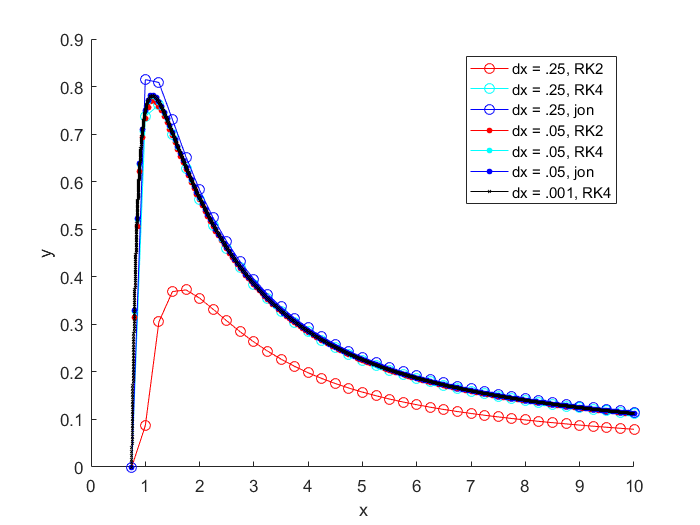
\includegraphics[scale=.75]{ex5_fig.png} 
			\caption{Comparison of several RK techniques.}
			\label{fig:RK2RK4RKjon}
		\end{figure}
	\end{center}
Notice that the RK4 scheme performs relatively well, even with a large step size of .25. This is the power of predictor corrector techniques - it overcomes inaccuracies caused by sharp curvature by considering the slope at various points. In this example, we see that the RK2 technique does not have enough prediction/correction steps to overcome the curvature. The jon's method is better than the RK2 method but worse than RK4. This is not surprising - it has one more prediction and correction step than RK4, but the sampling points and weighting was chosen arbitrarily instead of so as to minimize the error.
	\subsection{Adaptive Step Sizes}
	For most of the methods considered so far, it was assumed that a uniform step size was used. In most cases, this is a very natural and reasonable choice to make. However, for problems that are very computationally expensive and take a long period of time to run, efficiency becomes very important so as to reduce the number of steps needed. One of the best ways to do this is to use a step size that changes. While there are various rules for choosing the step size, the basic idea is to check the error at each step and to make it smaller if the error is to large.
	\subsubsection{Richardson Extrapolation}
	In this context, suppose that we are trying to solve a given IVP with a method that is $k$ order accurate. Let $A^*$ represent the exact solution. We have
	\begin{align}
		A^* &= A(h) + Bh^k + Ch^{k+1} \nonumber \\
		&= A(h) + Bh^k + \mathcal{O}(h^{k+1}) \label{rich1}
	\end{align}
	where $A(h)$ is the approximate solution from the scheme with step size $h$ and $B$ is a constant. Going forward, we will sometimes neglect writing the higher order terms because they are (hopefully) sufficiently small, but do not forget that they are always there. Multiplying both sides by $2^k$ and using a step size of $\frac{h}{2}$ 
	\begin{equation}
		2^k A^* = 2^k A\left(\frac{h}{2}\right) + B h^k \label{rich2} + \mathcal{O}(h^{k+1})
	\end{equation}
	subtracting \eqref{rich2} - \eqref{rich1}
	\begin{gather}
		(2^k -1)A^* = 2^k A\left(\frac{h}{2}\right) - A(h) + \mathcal{O}(h^{k+1}) \nonumber \\
		A^* = \frac{2^k A\left(\frac{h}{2}\right) - A(h)}{(2^k -1)} + \mathcal{O}(h^{k+1}) \label{rich3}
	\end{gather}
	what this says is that when integrating a differential equation, if we make two predictions  for $y_{n+1}$ with a step size $h$ (one step) and $\frac{h}{2}$ respectively, we can use \eqref{rich3} to get an approximation that is $k+1$ accurate, an entire order more accurate than $A(h)$ and $A(\frac{h}{2})$. This is useful, but we still need to determine if it is \textit{good enough}. To determine this, we can compute the error of $A(\frac{h}{2})$, which we know will be $\textit{less}$ accurate than \eqref{rich3}. If this error is good enough, than the error from \eqref{rich3} will certainly be good enough.
	\begin{align}
		E_{rr}[A(h/2)] &= A^* - A(h/2) \nonumber \\
		&= B(h/2)^{k} + \mathcal{O}(h)^{k+1}		 \nonumber \\
		&= B(h/2)^k  \label{rich4}
	\end{align}
	Now solving for $B$
	\begin{gather*}
		A^* = A(h) + Bh^k + Ch^{k+1} \\
		A^* = A(h/2) + B(h/2)^k + C(h/2)^{k+1}
	\end{gather*}
	subtracting these two equations
	\begin{gather}
		0 = A(h) - A(h/2) + Bh^k (1 - \frac{1}{2^k}) + \mathcal{O}(h^{k+1}) \nonumber \\
		B = \frac{A(h) - A(h/2)}{h^k (1 - \frac{1}{2^k})} + \mathcal{O}(h^{k+1}) \label{rich5}
	\end{gather}
	plugging \eqref{rich5} into \eqref{rich4}
	\begin{equation}
		E_{rr}[A(h/2)] = \frac{A(h) - A(h/2)}{\frac{1}{2^k} - 1} \label{rich6}
	\end{equation} 
	With all this, we can now describe a method for integrating with an adaptive step size:
	\begin{enumerate}
		\item Start with a set step size $h$. Compute $A(h)$ and $A(h/2)$. In other words, compute $y_{n+1}$ twice: once with step size $h$, and again with step size $(h/2)$ (this one will take two steps to reach $y_{n+1}$.
		\item Calculate the error using \eqref{rich6} and compare it to your error tolerance. If the error is less than the tolerance, calculate $y_{n+1}$ from $A(h)$ and $A(h/2)$ using \eqref{rich3}.
		\item If the error is greater than the tolerance, the integration will need to be repeated with a new timestep. If the error was within the tolerance, a new timestep for the next step should be predicted. In either care, the new step size can be estimated by solving
		\[
			E_{rr} [A(h)] = Bh_{new,1}^k
		\]
		\item Either repeat the previous integration or move onto the next one using 
		\[
			h_{new,2} = .9 h_{new,1}
		\]
		where the factor of .9 is added to help ensure that the desired accuracy is reached.
		\end{enumerate}
		\begin{exmp}
			Given $y'(x) = (.01x^2-2)y^{.5} + e^{-x^2}y + x^2\sin^2(x)$ and the initial condition $y(2) = 0$, use an adaptive step to calculate $y(10)$. Compare the results to using a uniform step size.
		\end{exmp}
	\textbf{Solution}
		\begin{figure}[H]
		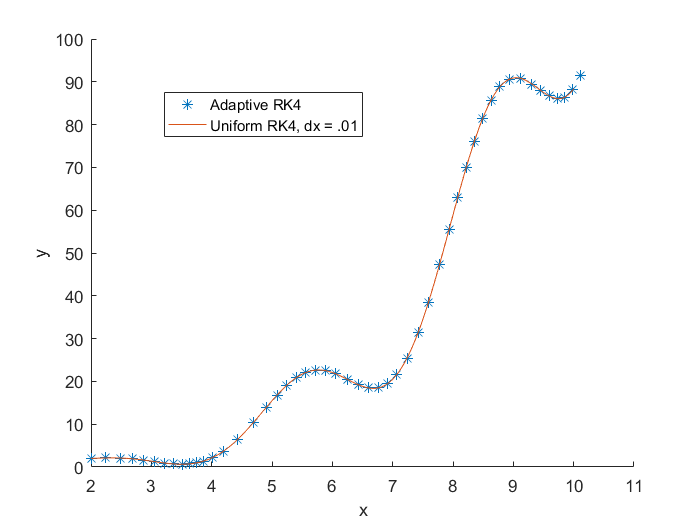
\includegraphics[scale=.7]{ex6_fig.png} 
		\caption{Comparison of adaptive and uniformly spaced RK4 method.}
		\label{fig:AdapRK4}
		\end{figure}
	From Figure \ref{fig:AdapRK4}, we see that the adaptive RK4 method is able to ensure very high accuracy while making much larger step sizes. Notice that as the curvature increases, the step size becomes smaller, and when the curvature decreases the step size becomes bigger. Although each step of the adaptive algorithm involves more computations than a single step of a uniform RK4 method, the total number of computations is much lower overall.
		\lstinputlisting{ex6.m}
		
	
	\subsection{Higher Order Differential Equations}
	\subsection{Direct explicit methods}
	Many of the lessons from previous sections are still for higher order differential equations. We can convert the equation into a discrete scheme with derivative approximations, and then either solve it with an explicit or implicit method. Since there is essentially nothing new to learn, it is best to start with an example.
	\begin{exmp}
		Solve $x^2y''(x) + xy'(x) + (x^2-4)y = 0$ on the interval $ 1 \leq x \leq 10 $ subject to the conditions $y(1) = .75$, $y'(1) = 1$. Use centered difference quotients and an explicit scheme.
	\end{exmp}
	\textbf{Solution:} First, we write the discrete form of the equation and isolate for $y_{n+1}$
	\begin{align*}
		&x^2 \frac{y_{n+1} - 2y_n + y_{n-1}}{\Delta x^2} + x \frac{y_{n+1}-y_{n-1}}{2\Delta x} + (x^2-4)y_n = 0 \\
		&y_{n+1} - 2y_n + y_{n-1}  + \left(\frac{\Delta x}{x}\right) \frac{y_{n+1}-y_{n-1}}{2} + \left(\frac{\Delta x^2}{x^2}\right)(x^2 - 4) y_n = 0 \\
		&\left(1 + \frac{\Delta x}{2x}\right)y_{n+1} = \left(\frac{4\Delta x^2}{x^2}-\Delta x^2 + 2\right) y_n + \left(\frac{\Delta x}{2x} -1 \right) y_{n-1} \\
		&y_{n+1} = \frac{\frac{4\Delta x^2}{x^2}-\Delta x^2 + 2}{1 + \frac{\Delta x}{2x}} y_n + \frac{\frac{\Delta x}{2x} -1}{1 + \frac{\Delta x}{2x}}y_{n-1}
	\end{align*}
	We are given $y_0$, but we also need $y_1$ or $y_{-1}$. The second boundary condition gives us an additional equation if we use a forward quotient:
	\begin{align*}
	&\frac{y_1 - y_0 }{\Delta x} = y'(0) \\
	&y_1 = y_0 + \Delta x y'(0) \\
	&y_1 = .75 + \Delta x
	\end{align*}
	\begin{center}
	\begin{figure}[H]
		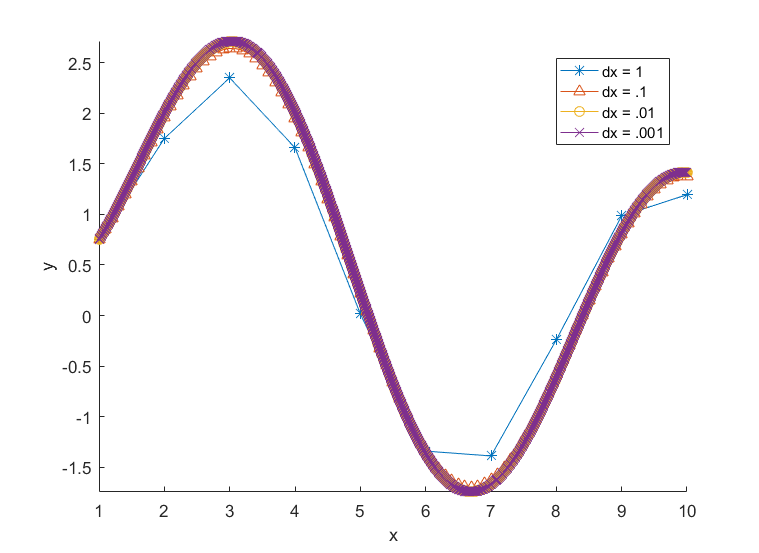
\includegraphics[scale=.75]{2_2fig.png} 
		\caption{Centered scheme with various timesteps.}
		\label{fig:num_bessel_fig}
	\end{figure}
	\end{center}
	From Figure \ref{fig:num_bessel_fig}, we see that convergence is achieved rather quickly. Although the final expression is rather cumbersome, the process was virtually identical to that used for a first order ODE.
	\begin{exmp}
		Given the equation $\frac{y''(x)}{1+x^2} - \sin(x)y'(x) + (x^2 - 1)y(x) = 0$ and the boundary conditions $y(1) = y(4) = 0$, find $y(x)$ on the interval $ 1 \leq x \leq 4$. 
	\end{exmp}
	\textbf{Solution} We begin by writing the corresponding discrete equation. For simplicity, we will use centered difference schemes.
	\begin{gather*}
		\frac{y_{n+1} - 2y_n + y_{n-1}}{(1+x_n^2)\Delta x^2} - \sin(x_n) \frac{y_{n+1} - y_{n-1}}{2\Delta x} + (x_n^2 -1) y_n = 0 \\
		\left(\frac{1}{(1+x_n^2)\Delta x^2} - \frac{\sin(x_n)}{2\Delta x}\right) y_{n+1} + \left(x^2_n -1 - \frac{2}{(1+x_n^2)\Delta x^2}\right) y_n + \left(\frac{1}{(1+x_n^2)\Delta x^2} + \frac{\sin(x_n)}{2\Delta x}\right) y_{n-1} = 0 \\
		y_{n+1} = \frac{\left(-x^2_n +1 + \frac{2}{(1+x_n^2)\Delta x^2}\right)}{\left(\frac{1}{(1+x_n^2)\Delta x^2} - \frac{\sin(x_n)}{2\Delta x}\right)} y_{n} - \frac{\left(\frac{1}{(1+x_n^2)\Delta x^2} + \frac{\sin(x_n)}{2\Delta x}\right)}{\left(\frac{1}{(1+x_n^2)\Delta x^2} - \frac{\sin(x_n)}{2\Delta x}\right) } y_{n-1}
	\end{gather*}
	Because the boundary conditions do not allow us to get two consecutive values for $y_k$ and $y_{k+1}$, we will have to solve this system as a matrix. For convenience, suppose 
	\[
		y_{n+1} = f_1(x_n) y_{n} - f_2(x_n)y_{n-1}
	\]
	 with $f_1,f_2$ being the appropriate functions just derived. We see that we if we divide the interval $[1,4]$ into $N$ points, we can write $N-2$ equations:
	 \begin{align*}
	 	f_2(x_1)y_0-f_1(x_1) y_1 +y_2 &= 0 \\
	 	f_2(x_2)y_1-f_1(x_2) y_2  + y_3&=0 \\
	 	f_2(x_3)y_2 - f_1(x_3)y_3 + y_4 &= 0 \\
	 	&\vdots  \\
	 	f_2(x_{N-2})y_{N-3} - f_1(x_{N-2})y_{N-2} + y_{N-1} &= 0
	 \end{align*}
	 Notice that we only have $N-2$ equations but $N$ variables. The final two equations from the boundary condition give us enough information to solve the system of equation. Given this, we can rewrite the system of equations as a matrix equation:
	\[\begin{bmatrix}
		f_2(x_1) & -f_1(x_1) & 1 & 0 & 0 & 0 & 0 &\ldots \\
		0 & f_2(x_2) & -f_1(x_2) & 1 & 0 & 0 & 0 &\ldots \\
		0 & 0 & f_2(x_3) & -f_1(x_3) & 1 & 0 & 0 &\ldots \\
		\vdots & \vdots & \vdots & \vdots & \vdots & \vdots & \ddots
	\end{bmatrix}
	\begin{bmatrix}
	y_0 \\
	y_1 \\
	y_2 \\
	y_3 \\
	y_4 \\
	\vdots \\
	y_{N-1}
	\end{bmatrix}
	= \begin{bmatrix}
	0 \\
	0 \\
	0 \\
	0 \\
	0 \\
	\vdots \\
	0
	\end{bmatrix}
	\]  
	Thus, solving  the problem now reduces to solving this matrix equation. 
		\begin{center}
		\begin{figure}[H]
			\centering
			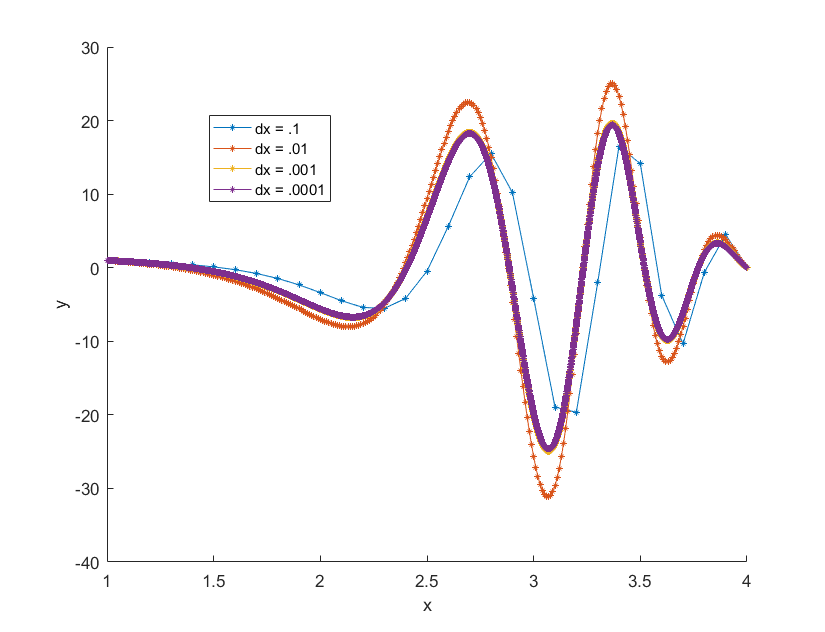
\includegraphics[scale=.7]{ex7_fig.png} 
			\caption{Centered scheme with various timesteps.}
			\label{fig:2ndorder2}
		\end{figure}
	\end{center}
\lstinputlisting{ex7.m}
\subsection{Conversion into a system of equations}
The more standard way of solving higher order linear ordinary differential equation is to use a transformation of variables. Suppose we are given the equation
\begin{equation}
	f_0(x) \frac{\diff^n y}{\diff x^n}  + f_1(x) \frac{\diff^{n-1}y}{\diff x^{n-1}} + \ldots + f_{n-2}(x) \frac{\diff^2y}{\diff x^2} + f_{n-1}(x) \frac{\diff y}{\diff x} + f_{n}(x) = 0
\end{equation}
Consider the transformation
\begin{align*}
	v_0 &= y \\
	v_1 &= \frac{\diff y }{\diff x} \\
	v_2 &= \frac{\diff^2 y}{\diff x^2} \\
	&\vdots \\
	 v_{n-2} &= \frac{\diff^{n-2}y}{\diff x^{n-2}}  \\
	 v_{n-1} &= \frac{\diff^{n-1}y}{\diff x^{n-1}}
\end{align*}
Upon taking the derivative of each $v_i$ term, we see that the problem is now transformed into solving a system of first order differential equations. Observe that the differential equation for each $v_i$ term is almost trivial to write except for the last one. For this derivative, we use the original differential equaiton itself to obtain the corresponding term.
\begin{gather*}
	v_0' = v_1 \\
	v_1' = v_2 \\
	v_2' = v_3 \\
	 \vdots \\
	v_{n-2}' = v_{n-1} \\
	v_{n-1}' = \frac{-f_n(x)}{f_0(x)} - \frac{f_{n-1}(x)}{f_0(x)} v_1 - \frac{f_{n-2}(x)}{f_0(x)} v_2 - \ldots - \frac{f_1(x)}{f_0(x)} v_{n-1}
\end{gather*}
Or, expressed in matrix form
\begin{equation*}
	\underbrace{\begin{bmatrix}
	v_0 \\
	v_1 \\
	v_2 \\
	\vdots \\
	v_{n-2} \\
	v_{n-1} 
	\end{bmatrix}'}_{\mathbf{v'}} =
	\underbrace{\begin{bmatrix}
	0 &1  & 0 & 0 &0 &  \ldots & 0  \\
	0 & 0 & 1 & 0 & 0  & \ldots & 0\\
	0 & 0 & 0 & 1 & 0 & \ldots &0 \\
	\vdots & \vdots & \vdots  & \vdots & \ddots & &  \vdots\\
	0 & 0 & 0 & 0 & 0 & \ldots & 1 \\  
	\frac{-f_{n-1}}{f_0} & \frac{-f_{n-2}}{f_0} & \ldots &  \ldots & \ldots & & \frac{-f_{1}}{f_0} \\
	\end{bmatrix}}_{\mathbf{A}}
	\underbrace{\begin{bmatrix}
		v_0 \\
	v_1 \\
	v_2 \\
	\vdots \\
	v_{n-2} \\
	v_{n-1} 
	\end{bmatrix}}_{\mathbf{v}} + 
		\underbrace{\begin{bmatrix}
	0 \\
	0 \\
	0 \\
	\vdots \\
	0 \\
	\frac{-f_n}{f_0} 
	\end{bmatrix}}_{\mathbf{b}}
\end{equation*}
From here, any appropriate method can be used to solve for $v_0$, which will also be a solution to the original differential equation.
\begin{exmp}
	Given the IVP problem $y''' -2x^2 y'' + xy' = 0$ and the initial conditions $y(0) = 0$,  $y'(0) = 6$, $y''(0)=-5.5$, solve for y(12).
\end{exmp}
\textbf{Solution:} Using the transformations
\begin{align*}
	v_0 &= y \\
	v_1 &= y' \\
	v_2 &= y'' \\
\end{align*}
recasting the equation using the new variables
\begin{align*}
	v_0' &= v_1, \quad v_0(0) = 0\\
	v_1' &= v_2, \quad v_1(0) = 0\\
	v_2' &= 2x^2v_2 - xv_1, \quad v_2(0) = 0
\end{align*}
which can be easily integrated using an RK4 method.
		\begin{center}
	\begin{figure}[H]
		\centering
		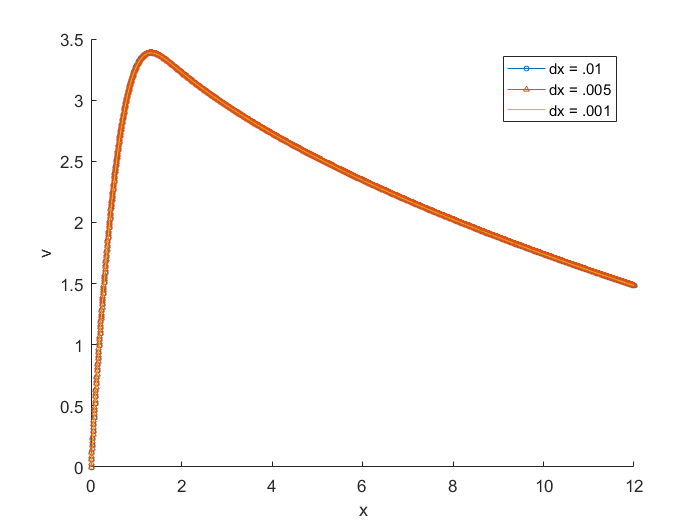
\includegraphics[scale=.7]{ex8_fig.png} 
		\label{fig:system1}
	\end{figure}
\end{center}
\lstinputlisting{ex8.m} The previous example had initial data that was nice - we did not have to jump through any hoops to incorporate it. However, this is not always the case, as the following example will illustrate. If we are given initial data located at different points, we end up having to solve a matrix equation rather than just a recurrence relation.
\begin{exmp}
	Given $y''+\frac{1}{x}y'+ (x+1)y = 0$ and the boundary conditions $y(0) = 1$, $y(20) = 25$, find $y(5)$.
\end{exmp}
\textbf{Solution:} We begin by making the transformation $v_0 = y$ and $v_1 = y'$ to obtain 
\begin{align*}
	v_0' &= v_1 \\
	v_1' &= -(x+1)v_0 - \frac{1}{x}v_1
\end{align*}
\[
	\underbrace{\begin{bmatrix}
	v_0 \\
	v_1
	\end{bmatrix}'}_{\mathbf{v'}} = \underbrace{\begin{bmatrix}
	0 & 1 \\
	-(x+1) & \frac{-1}{x} \\
	\end{bmatrix}}_{\mathbf{A}} \underbrace{\begin{bmatrix}
	v_0 \\
	v_1 
	\end{bmatrix}}_{\mathbf{v}}
\]
which can be solved with an RK4 scheme. Notice now that we are working with vectors instead of scalars. Letting $\mathbf{A}_n = \mathbf{A}|_{x=x_n}$,
\begin{align*}
	\mathbf{h}_1 &= dx \mathbf{A}_n \mathbf{v}_n \\
	\mathbf{h_2} &= dx\mathbf{A}_{n+.5} (\mathbf{v}_n + .5\mathbf{h}_1)
\end{align*}
\end{document}

%%references: 
% https://people.sc.fsu.edu/~jpeterson/nde_book4.pdf
%http://www.math.ubc.ca/~feldman/m256/richard.pdf
